% concatenated from revised2_pra.tex
% ****** Start of file apssamp.tex ******
%
%   This file is part of the APS files in the REVTeX 4.2 distribution.
%   Version 4.2a of REVTeX, December 2014
%
%   Copyright (c) 2014 The American Physical Society.
%
%   See the REVTeX 4 README file for restrictions and more information.
%
% TeX'ing this file requires that you have AMS-LaTeX 2.0 installed
% as well as the rest of the prerequisites for REVTeX 4.2
%
% See the REVTeX 4 README file
% It also requires running BibTeX. The commands are as follows:
%
%  1)  latex apssamp.tex
%  2)  bibtex apssamp
%  3)  latex apssamp.tex
%  4)  latex apssamp.tex
%
\documentclass[reprint, amsmath,amssymb, aps,pra,
 floatfix,
]{revtex4-2}
% \documentclass[floatfix]{revtex4-2}
% \documentclass[aps,pra]{revtex4-2}

\usepackage[caption=false]{subfig} % works well with revtex4-2
\usepackage{bm}
\usepackage[dvipsnames]{xcolor}
\usepackage[pdftex]{graphicx}% Include figure files
\usepackage{dcolumn}% Align table columns on decimal point
\usepackage{bm}% bold math
% \usepackage{cite}
% \usepackage{xcolor}
\usepackage{tikz}
\usepackage{amsthm}
% \usepackage{algorithmic}
\usepackage[linesnumbered,ruled,vlined]{algorithm2e}  % For algorithms
\usepackage{algpseudocode}  % For pseudocode
\usepackage{graphicx}
% \usepackage{subcaption}
\newtheorem{theorem}{Theorem}
\newtheorem{lemma}[theorem]{Lemma}
\newtheorem{corollary}[theorem]{Corollary}
\newtheorem{remark}{Remark}
\usepackage{quantikz}
\usepackage[table]{xcolor}
\usepackage{colortbl} % optional
\usepackage{graphicx} % for \resizebox
% \usepackage{tcolorbox} 
% \usepackage{graphicx}
% \usepackage{textcomp}

% \usepackage{jabbrv}
\usepackage[normalem]{ulem}

% for the plot package
% \usepackage{fontspec}
% \setmainfont{Arial}
% \usepackage{newtxtext,newtxmath}
\usepackage{pgfplots}
\pgfplotsset{compat=1.18}

% \usepackage{pgfplots}
% \pgfplotsset{
%     compat=1.18,
%     every axis/.append style={
%         font=\bfseries
%     }
% }
%\usepackage[mathlines]{lineno}% Enable numbering of text and display math
%\linenumbers\relax % Commence numbering lines

%\usepackage[showframe,%Uncomment any one of the following lines to test 
%%scale=0.7, marginratio={1:1, 2:3}, ignoreall,% default settings
%%text={7in,10in},centering,
%%margin=1.5in,
%%total={6.5in,8.75in}, top=1.2in, left=0.9in, includefoot,
%%height=10in,a5paper,hmargin={3cm,0.8in},
%]{geometry}
\SetKwInput{KwInput}{Input} 
\SetKwInput{KwOutput}{Output}  
\SetKwInput{KwInit}{Initialization}   
\SetKwInput{KwStep}{Step1}
\SetKwInput{KwStepp}{Step2}
\SetKwInput{KwSteppp}{Step3}

\newcommand{\PadCell}[1]{\kern8pt#1\kern8pt}
\newcommand{\PadCellColor}[2]{\cellcolor{#1}\kern8pt#2\kern8pt}

\usepackage{hyperref}% add hypertext capabilities
\hypersetup{
  colorlinks   = true, % Colours links instead of ugly boxes
  urlcolor     = blue, % Colour for external hyperlinks
  linkcolor    = blue, % Colour of internal links
  citecolor    = blue  % Colour of citations
}

\begin{document}

\preprint{APS/123-QED}

\title{Fault-tolerant syndrome extraction in \texorpdfstring{$[[n,1,3]]$}{[[n,1,3]]} non-CSS code family generated using measurements on graph states}

\author{Harsh Gupta}
\email{harsh22@iiserb.ac.in}
 \affiliation{
 Department of Electrical Engineering and Computer Science, Indian Institute of Science Education and Research Bhopal, 462066 Bhopal, India }
\author{Mainak Bhattacharyya}
 \email{mainak23@iiserb.ac.in}
\affiliation{
 Department of Electrical Engineering and Computer Science, Indian Institute of Science Education and Research Bhopal, 462066 Bhopal, India }
\author{Ritik Jain}
 \email{ritikjain@iiserb.ac.in}
\affiliation{
 Department of Electrical Engineering and Computer Science, Indian Institute of Science Education and Research Bhopal, 462066 Bhopal, India }
\author{Ankur Raina}
 \email{corresponding author: ankur@iiserb.ac.in}
\affiliation{
 Department of Electrical Engineering and Computer Science, Indian Institute of Science     Education and Research Bhopal, 462066 Bhopal, India }

\date{\today}

\begin{abstract}
\noindent The reliability of quantum computation critically depends on the performance of quantum error-correcting codes (QECCs).
Performance of QECCs can be severely degraded by hook errors, which effectively reduce the code distance.
In this work, we construct a family of $[[n,1,3]]$ non-CSS QECCs, which are fault-tolerant (FT) against noisy syndrome measurements.
We employ the bare-ancilla method of Muyuan Li \emph{et al.} to demonstrate fault tolerance against hook errors during syndrome extraction.
We present a systematic protocol for generating these QECCs using graph codes and propose a family of $[[n,1,3]]$ codes that preserve the fault-tolerant properties of the bare ancilla codes.
We use a custom lookup-table decoder and simulate the code's performance under both anisotropic and circuit-level depolarizing noise.
Our results reveal a trade-off in performance with respect to the code rate and identify optimized codes under these noise models.
We benchmark our results against the flag-qubit method of Chao \emph{et al}.
Notably, we report a new bare ancilla code with improved code rate while maintaining the same distance compared to the bare code used in the work of Muyuan Li \emph{et al.}
\end{abstract}

\keywords{Fault Tolerance, Non-CSS Quantum codes, Hook Errors, Bare Ancilla, Flag error correction.}
\maketitle

\section{Introduction}
\label{sec:introduction}

\noindent The evolution of hardware architectures for quantum computing has been rapid in recent years to support a reliable fault-tolerant framework for the quantum protocols.
Manipulation of the logical information encoded on the physical qubits should yield high fidelity, indicating highly error-suppressed outcomes.
As a result, the development of a robust Quantum Error Correcting Code (QECC) is fundamental in the advancement of fault-tolerant (FT) quantum computing.
Implementing QECCs in practical scenarios poses significant challenges, particularly due to physical errors that affect the error detection process. 
During a computation, fault tolerance can be achieved asymptotically if the physical error rate is below a certain threshold~\cite{10.1145/258533.258579, nielsen2010quantum}.
Crucially, the syndrome extraction process must also be implemented in an FT manner to prevent errors from propagating into the data qubits.
One of the earliest codes tested for fault tolerance on small systems is the  $[[4,2,2]]$ QECC using ion trap and superconducting qubits \cite{10.5555/3370220.3370224, PhysRevLett.119.180501}. They demonstrated that error detection can improve certain simple sampling tasks. 
This code only detects a Pauli error as its minimum distance is two.
Any limited error-correcting capacity of a QECC imposes significant resource overhead required for FT quantum computation.
Several techniques have been proposed for extracting FT syndrome.
Steane's method requires an FT logical state in the syndrome measurement, whereas Shor's method requires extra qubits prepared in the cat state for FT syndrome measurement~\cite{PhysRevLett.78.2252,shor1996}.
Similarly, Knill's method uses a logical Bell pair~\cite{Knill2005}.\\\\
\noindent Researchers have shown that stabilizers outside the minimal generating set can be leveraged to strengthen the error-correcting capability of quantum codes~\cite{fujiwara2015high}.
Fujiwara proved that it is possible to detect the measurement error of the syndrome qubit even in $[[5, 1, 3]]$ QECC~\cite{fujiwara2014ability}.
Yoder \emph{et al.} address that both $[[5,1,3]]$ and $[[7,1,3]]$ QECCs can be made resistant to hook errors using three and two additional qubits, respectively~\cite{Yoder2017surfacecodetwist}. 
Using an extra two qubits, Chao and Reichardt were able to correct the faults of distance-three codes that lead to correlated errors in data qubits during syndrome extraction~\cite{PhysRevLett.121.050502}.
Muyuan Li \emph{et al.} proposed the bare method, a FT syndrome-extraction scheme for a $[[7,1,3]]$ QECC that uses only one ancillary qubit by cleverly reordering the stabilizer's operators.
This method ensures no logical error occurs in data qubits due to a single Pauli error on the ancillary qubit~\cite{Muyuna}.
The authors in Ref. \cite{Muyuna} find the logical error rates for anisotropic noise below the pseudo-threshold limit. 
The procedure by which this specific $[[7,1,3]]$ code is identified is not explicitly described.
This observation motivates a systematic search for the family of $[[n,1,3]]$ QECCs, which supports FT syndrome extraction using the bare method. 
In addition, we explore QECCs with improved code rates that similarly prevent hook errors caused by a single Pauli error on the ancillary qubit.\\\\
\noindent In this work, we derive explicit syndrome-space conditions under which stabilizer codes support bare-ancilla fault-tolerant syndrome extraction, thereby identifying a class of bare ancilla codes (BACs).
To the best of our knowledge, such general bounds for BAC constructions have not previously been established.
We then introduce a systematic framework for constructing non-CSS BACs from graph-codes and show how suitable stabilizer measurement orderings remove hook-error degeneracies using only a single bare ancilla qubit~\cite{Schlingemann_2001, PhysRevA.69.022316,cafaro:hal-02287093,schlingemann2001stabilizercodesrealizedgraph}.
Using this framework, we construct a new family of \([[n,1,3]]\) BACs that enable fault-tolerant syndrome extraction without additional verification or flag qubits~\cite{PhysRevLett.121.050502}.
We evaluate these codes under anisotropic and circuit-level depolarizing noise and benchmark them against the flag-qubit approach.
The simulations show that the proposed BACs provide competitive, and in several cases improved, logical-error performance while requiring fewer ancillary resources.\\
\noindent The paper is structured as follows. In Sec.~\ref{sec:Preliminaries}, we discuss the Calderbank-Shor-Steane (CSS) and non-CSS QECCs, along with the review of techniques used to make  QECCs FT during syndrome measurement. 
The graph code construction using a parity-check matrix is given in Sec.~\ref{sec: MBQC construct QECC}, which will be used for BAC construction.
In Sec.~\ref{sec: Bare constrcution}, we present an algorithm to construct a BAC given a non-CSS stabilizer with the existence proof of family a of $[[n,1,3]]$ bare code using graph codes.
Experimental setup with noise models is discussed in Sec.~\ref{sec:experimental setup}.
Simulation results, which include logical error rate comparison of BAC and flag method, are reported in Sec.~\ref {sec:results analysis}.
We conclude the paper in Sec .~\ref {sec:conclusion}.
\section{Background and Preliminaries}
\label{sec:Preliminaries}
\noindent QECCs form the foundation for protecting quantum information against decoherence and operational errors.
We shall briefly discuss some basic concepts necessary to understand the rest of the paper in this section.
\subsection{CSS and non-CSS codes}

\noindent In 1995, Shor introduced the first scheme capable of correcting arbitrary single-qubit errors using nine physical qubits, achieving a code rate of $1/9$~\cite{shor9qubit1995}.
Steane subsequently introduced a seven-qubit code with a higher code rate of $1/7$~\cite{steane1996}.
Laflamme \emph{et al.} later established the five-qubit ``perfect'' code, which saturates the quantum Hamming bound and achieves the minimum block size required to protect a single logical qubit from any single-qubit error~\cite{laflamme1996perfect}.
While these codes differ in code length, they share the same minimum distance and therefore exhibit equivalent error-correction capability.
This line of work can be unified under the stabilizer formalism, where an $[[ n,k,d]]$ stabilizer code is defined as the joint $+1$ eigenspace of an Abelian subgroup $ \mathcal{S}$ of the Pauli group $P_n$ on the Hilbert space $(\mathbb{C}^2)^{\otimes n}$~\cite{gottesman1997stabilizercodesquantumerror}.
A key subclass is formed by Calderbank-Shor-Steane (CSS) codes, which are constructed from two classical linear codes with parity-check matrices $\mathbf{H}_\mathrm{x}$ and $\mathbf{H}_\mathrm{z}$ such that $C_Z^\perp \subseteq C_X$ and $C_X^\perp \subseteq C_Z$~\cite{Calderbank_1996}.
CSS codes address bit-flip and phase-flip errors independently, while non-CSS codes handle both simultaneously~\cite{laflamme1996perfect}.
In addition, non-CSS codes are not restricted by the structural constraints that govern CSS code design and have the potential to exceed the performance limits of CSS schemes and approach the hashing bound of a quantum channel~\cite{noncsshashingbound}.
Algebraically for a stabilizer code with parity check matrix $\mathbf{H=[H_\mathrm{x}|H_\mathrm{z}]}$, the following relation holds 
\begin{align}
 \mathbf{H_\mathrm{z} H_\mathrm{x}^T+ \ H_\mathrm{x} H_\mathrm{z}^T = \mathbf{0}}.
  \label{eq:18}
\end{align} 
Equation \ref{eq:18} is the symplectic commutation condition that guarantees mutual commutativity among the stabilizer generators.
This condition forms the algebraic foundation of both CSS and non-CSS stabilizer codes and ensures that syndrome measurements can be performed
consistently.
However, satisfying the stabilizer commutation relations alone is insufficient for achieving fault tolerance during syndrome extraction.
In practical implementations, faults on ancillary qubits may propagate via two-qubit interactions and generate correlated errors on the data qubits, commonly known as hook errors.
\subsection{Hook Errors in QEC}
\noindent Syndrome measurements in quantum error correction are typically performed by coupling ancilla qubits to several data qubits through two-qubit controlled gates such as $\mathrm{CNOT}$ or $\mathrm{CZ}$ gates~\cite{nielsen2010quantum}.
Pauli errors that occur on the ancilla qubit can propagate through these interactions and generate correlated errors on the data qubits.
They are called hook errors, since a single ancilla fault can effectively hook onto multiple qubits instead of remaining confined to one~\cite{10.1063/1.1499754}. Hence, a single physical fault in a syndrome qubit propagates to the data qubit and converts into two or more qubit errors. Therefore, meticulous circuit design is important to evade hook errors.
If left untreated, hook errors reduce the effective code distance and can significantly limit the code's error-correcting capability.
Consequently, fault-tolerant syndrome extraction requires circuit-level mechanisms that either suppress hook-error propagation, detect its occurrence, or ensure that the resulting propagated errors remain uniquely decodable.
This requirement motivates the fault-tolerant syndrome-extraction schemes reviewed next.

\subsection{Fault-tolerant syndrome-extraction schemes}

\noindent Over the past decade, major advances have been made in developing fault-tolerant schemes for syndrome measurement.
Fujiwara identified a previously unrecognized property of stabilizers in quantum error-correcting codes~\cite{fujiwara2014ability}.
He demonstrated that using combinations of stabilizers outside the minimal generating set, traditionally considered redundant, can enhance the error-correcting capability of the stabilizer code.
Building on this idea, Ashikhmin \emph{et al.} generalized existence theorems and extended the quantum singleton bound to incorporate measurement redundancy~\cite{ashikhmin2014robust}.
Crow \emph{et al.} showed that redundant stabilizers can result in error thresholds comparable to those of conventional measurement-based methods without explicit measurement, often called measurement-free quantum error correction~\cite{crow2016improved}.
Subsequently, various approaches have been proposed to exploit redundancy in syndrome extraction, though these techniques primarily address errors in syndrome qubit measurements~\cite{premakumar20212,guttentag2024robust}.\\\\
\noindent Yoder and Kim demonstrated that hook errors arising from interactions between syndrome qubits and data qubits can also be corrected via a suitably designed framework, with a significant overhead~\cite{Yoder2017surfacecodetwist}.
Chao and Reichardt later addressed this issue by introducing a more resource-efficient scheme that requires only two additional qubits, an ancilla qubit, and a flag qubit~\cite{PhysRevLett.121.050502}.
This approach is applicable to all stabilizer codes~\cite{chamberland2017flag,chao2020flag}.
Subsequent work produced several variants of the flag-qubit method, optimizing circuit depth by dynamically and adaptively selecting stabilizer measurements and introducing tools to simulate and optimize the flag approach~\cite{debroy2020extended,bhatnagar2023low,WOS:001379568200001,WOS:001317800000001,pato2024optimization}.
Lao and Almudever extended this approach by introducing a geometrical interaction mapping~\cite{PhysRevA.101.032333}.
They combine fault-tolerant flagging with quantum circuit mapping to create an efficient flag-bridge implementation of FT quantum error correction on near-term devices.\\\\
\noindent Further improvement to overhead requirements was proposed by Muyuan Li \emph{et al.}.
They introduced a $[[7,1,3]]$  non-CSS stabilizer code, which utilises reordering of stabilizers and uses only one ancilla qubit while measuring the syndrome to achieve fault-tolerant capabilities against the hook errors~\cite{Muyuna}. 
They analyzed code performance under anisotropic and depolarizing noise and obtained a pseudo-threshold for anisotropic noise, a noise commonly encountered in trapped-ion systems~\cite{parrado2020crosstalk}. 
Researchers used a similar reordering method with a bare ancilla qubit to construct the FT syndrome measurement circuit for the Bacon-Shor code and compass codes ~\cite{PhysRevA.98.050301,huang2020fault}.
Maheshwari \emph{et al.}  analyzed a $[[8,1,3]]$ non-CSS QECC, reporting its pseudo-threshold under both depolarizing and anisotropic noise models using a bare ancilla qubit~\cite{maheshwari2024fault}.
Despite these advances in the bare-ancilla method, which reduce resource cost, their performance was tested on very limited codes.
Moreover, a systematic framework for constructing non-CSS stabilizer codes that mitigate hook errors while maintaining a higher code rate has yet to be developed.
Motivated by this gap, we construct a family of $[[n,1,3]]$ codes inspired by graph codes using a bare ancilla qubit for syndrome extraction.
The following section introduces graph codes, which serve as the foundation for our code construction.
\section{Non-CSS family of Quantum Code constructions using Measurements}

\label{sec: MBQC construct QECC}
\noindent We now discuss how the message information is encoded using measurements.
Stabilizer evolution under measurement is described using methods adapted from the Measurement-Based Quantum Computing (MBQC) setting.
\subsection{MBQC method}
\noindent MBQC was introduced by Raussendorf \emph{et al.}, which differs from the gate-based quantum computing models due to the measurement-based operations~\cite{PhysRevA.68.022312}.
Within this framework, quantum computation is carried out by first preparing and then entangling qubits into a highly structured resource state.
This so-called cluster or graph state is represented by an undirected graph $G = (V, E)$, shown in Figure \ref{fig: 2D cluster state}, where $V$  denotes the set of vertices corresponding to the qubits, and $E$ represents the edges corresponding to the $\mathrm{CZ}$ gates between the qubits.\\

\begin{figure}[htbp]
    \centering
    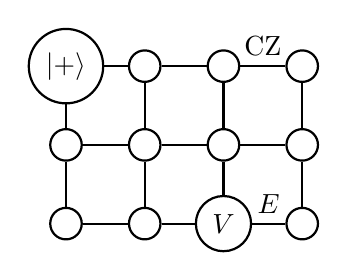
\begin{tikzpicture}[node distance={10mm}, thick, main/.style = {draw, circle, minimum size=0.4cm}]
\node[main] (1) {$|{+}\rangle$}; 
\node[main] (2) [ right of=1] {};
\node[main] (3) [right of = 2] {}; 
\node[main] (4) [right of= 3] {};
\node[main] (5) [below of = 1] {}; 
\node[main] (6) [below of= 2] {};
\node[main] (7) [below of = 3] {}; 
\node[main] (8) [below of = 4] {}; 
\node[main] (9) [below of = 5] {}; 
\node[main] (10) [below of = 6] {}; 
\node[main] (11) [below of = 7] {$V$}; 
\node[main] (12) [below of = 8] {}; 
\draw (1) -- node[midway, above right, sloped ] {} (2);
\draw (2) -- node[midway, above right, sloped ] {} (3);
\draw (3) -- node[midway, above , sloped ] {$\mathrm{CZ}$} (4);
\draw (5) -- node[midway, above right, sloped ] {} (6);
\draw (6) -- node[midway, above right, sloped ] {} (7);
\draw (7) -- node[midway, above right, sloped ] {} (8);
\draw (9) -- node[midway, above right, sloped ] {} (10);
\draw (10) -- node[midway, above right, sloped ] {} (11);
\draw (11) -- node[midway, above, sloped ] {$E$} (12);
\draw (1) -- node[midway, above right, sloped ] {} (5);
\draw (5) -- node[midway, above right, sloped ] {} (9);
\draw (2) -- node[midway, above right, sloped ] {} (6);
\draw (6) -- node[midway, above right, sloped ] {} (10);
\draw (3) -- node[midway, above right, sloped ] {} (7);
\draw (7) -- node[midway, above right, sloped ] {} (11);
\draw (4) -- node[midway, above right, sloped ] {} (8);
\draw (8) -- node[midway, above right, sloped ] {} (12);
\end{tikzpicture}
 \caption{A Cluster state, which is also depicted as an undirected graph $G=(V,E)$ where $V$ is the set of vertices corresponding to qubits, each initialized with $|{+}\rangle$ state and $E$ is the set of edges, each corresponding to a $\mathrm{CZ}$ gate.}   
 \label{fig: 2D cluster state}
\end{figure}

\noindent In order to move from the description of graph states to the construction of QECCs, it is important to recall how the measurement outcomes affect the stabilizer structure of a graph state.
The evolution of stabilizers under specific measurement choices provides the foundation for relating cluster states to error-correcting codes.
A formal derivation of the stabilizer generators of post-measurement states can be found in Ref. \cite{nielsen2010quantum}, while the detailed behavior of stabilizer sub-groups under various measurement settings is described in Ref. \cite{patil2023clifford,PhysRevA.69.062311}.
This perspective naturally motivates the construction of quantum error-correcting codes from graph states, known as graph codes.
The concept of graph codes was first introduced by Schlingemann and Werner, where the code space is defined through an isometry from input qubits to output qubits using a graph and a finite Abelian group~\cite{Schlingemann_2001,10.1007/978-3-642-20901-7_9}. 
Further, Schlingemann and Grassl \emph{et. al} independently showed that every stabilizer QECC can be represented as a graph code and vice versa~\cite{1023317,https://doi.org/10.48550/arxiv.quant-ph/0111080}. 

\noindent Graph codes defined in Ref. \cite{Schlingemann_2001,10.1007/978-3-642-20901-7_9} are also constructed using measurements on the message qubit.
When  $k$ message qubits are combined with $n$ qubits of the graph through $\mathrm{CZ}$ gates, we call it an $(n+k)$ qubit graph-message state.
Then encoding can be implemented by measuring the message qubits in the $X$ basis, as shown in Figure \ref{fig: encoding of message using MBQC}~\cite{hwang2015relationgraphcodegraph}.
\begin{figure}[ht]
    \centering
    
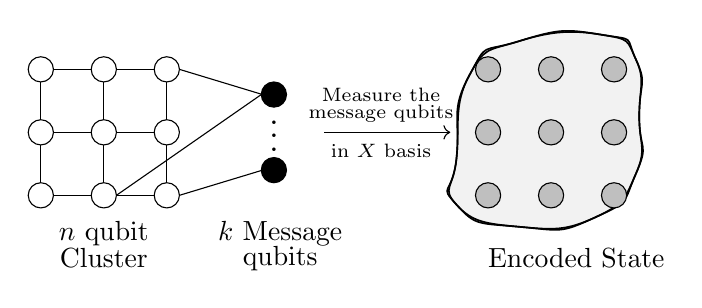
\begin{tikzpicture}[scale=0.8]
    % --------- Amoeba blob first (so it stays behind) ----------
    \fill[gray!10, draw=black, line width=0.6pt]
        plot[smooth cycle, tension=1.1] coordinates {
            (6.6,-0.15)
            (7.6,-0.5)
            (8.8,-0.35)
            (9.45,0.35)
            (9.5,1.25)
            (9.45,2.15)
            (8.9,2.55)
            (7.6,2.45)
            (6.8,1.9)
            (6.6,0.6)
        };

    % optional subtle darker border
    \draw[line width=0.6pt] 
        plot[smooth cycle, tension=0.9] coordinates {
            (6.6,-0.15)
            (7.6,-0.5)
            (8.8,-0.35)
            (9.45,0.35)
            (9.5,1.25)
            (9.45,2.15)
            (8.9,2.55)
            (7.6,2.45)
            (6.8,1.9)
            (6.6,0.6)
        };

    % --------- Left cluster grid (drawn on top of blob) ----------
    \foreach \x in {0,1,2} {
        \foreach \y in {0,1,2} {
            \draw (\x,\y) circle(0.2cm);
        }
    }
    \draw (0.2,0) -- (0.8,0);
    \draw (1.2,0) -- (1.8,0);
    \draw (0.2,1) -- (0.8,1);
    \draw (1.2,1) -- (1.8,1);
    \draw (0.2,2) -- (0.8,2);
    \draw (1.2,2) -- (1.8,2);
    \draw (0,0.2) -- (0,0.8);
    \draw (1,0.2) -- (1,0.8);
    \draw (2,0.2) -- (2,0.8);
    \draw (0,1.2) -- (0,1.8);
    \draw (1,1.2) -- (1,1.8);
    \draw (2,1.2) -- (2,1.8);
    \node at (1,-0.6){$n$ qubit};
    \node at (1,-1){Cluster};

    % --------- Message qubit ----------
    \draw[fill=black] (3.7,0.4) circle(0.2cm);
    \draw[fill=black] (3.7,1.6) circle(0.2cm);
    % \draw[fill=black] (3.8,1.7) circle(0.28cm);
    \draw (3.52,1.6) -- (2.2,2);
    \draw (3.52,0.4) -- (2.2,0);
    % \draw (3.5,1) -- (1.2,2);
    \draw (3.5,1.6) -- (1.2,0);
    \node at (3.7,1.1){$\scalebox{1.2}{$\vdots$}$};
    \node at (3.8,-0.6){$k$ Message};
    \node at (3.8,-1){qubits};

    \draw[->] (4.5,1) -- (6.5,1);
    \node at (5.4,1.6){\scriptsize Measure the};
    \node at (5.4,1.3){\scriptsize message qubits};
    \node at (5.4,0.7){\scriptsize in $X$ basis};

    % --------- Encoded state (3x3) coordinates (drawn after blob) ----------
    \foreach \i[count=\k] in {7.1,8.1,9.1} {
        \foreach \j in {0,1,2} {
            \draw[fill=gray!50] (\i,\j) circle(0.2cm);
        }
    }
    \node at (8.5,-1){Encoded State};
\end{tikzpicture}
   \caption{The message qubits (\Large\textcolor{black}{$\bullet$}\normalsize) are encoded into the cluster by measuring it in the $X$ basis.}
   \label{fig: encoding of message using MBQC}
   \end{figure}

\noindent Each stabilizer of the  $(n+k)$ qubit graph-message state is given by  Eq.~\eqref{eq:graph_state}:
\begin{align}
\label{eq:graph_state}
    g_j= X_j \prod_{i \in \mathcal{N}_j} Z_i, \, j \in \{1,2,\cdots, n\},
\end{align}
where $\mathcal{N}_j$ denotes the neighbours of the $j^{th}$ cluster qubit.
The parity check matrix corresponding to Eq. \eqref{eq:graph_state} can be written in an elegant form:
\begin{align}
   \mathbf{H}= [\mathbf{H}_\mathrm{x}\mid\mathbf{H}_\mathrm{z}]=[\mathbf{I}_{n\times n}:\mathbf{0}_{n\times k} \mid \mathbf{A}^{\mathrm{cc}}_{n\times n}:\mathbf{A}^{\mathrm{cm}}_{n\times k}],
  \label{eq:prof ankur equation}
\end{align}
where $\mathbf{A}^{\mathrm{cc}}_{n\times n}$ is an adjacency matrix associated with the cluster state of $(n+k)$ graph-message state \cite{8269075}. 
$\mathbf{A}^{\mathrm{cm}}_{n\times k}$ matrix indicates the connection of the message qubits to the cluster qubits. 
$\mathbf{I}_{n \times n}$ is the identity matrix and $\mathbf{0}_{n\times k}$ is the NULL matrix.\\
\noindent In this work, we use the same encoding procedure as shown in Figure \ref{fig: encoding of message using MBQC}, adopted from Ref. \cite{hwang2015relationgraphcodegraph}, whose formal proof is provided in Appendix~\ref{APPENDIX: MBQC min distance}. 
The encoded state is obtained by transformations to the parity-check matrix of the $(n+k)$ qubit graph-message state.

\subsection{Encoding of message qubits}

\noindent Let the generators of stabilizer group of $(n+k)$ qubit graph-message state be

\[
 \langle g_1,g_2, \cdots, g_{n-k} \rangle.
\]
To encode a message on the $(n+i)^{th}$ qubit, the stabilizer set is modified following the procedure in Ref. \cite{patil2023clifford}.
Algorithm-\ref{algo: matrix method} is the pseudo-code representation of these steps using a parity check matrix.
At each iteration, a pivot row with a ‘1’ in the \((n+i)^{\text{th}}\) column of \(\mathbf{H}_\mathrm{z}\) of message qubit is selected, and the pivot is added (modulo 2) to all other rows containing a ‘1’ in that column, thereby isolating the qubit in a single stabilizer.
The pivot row and the two columns corresponding to the measured qubit are subsequently removed. Repeating this procedure for all $k$ message qubits reduces the matrix dimension from $n$ $\times$ $2(n+k)$ to $(n-k)$ $\times$ $2n$, resulting in the stabilizer description of the encoded, generally non-CSS,  $[[n,k,d]]$ code in the MBQC framework.\\
{\linespread{1.05}\selectfont
\begin{algorithm}[H]
\DontPrintSemicolon
\caption{Graph code stabilizer construction via parity check matrix using measurements}
\label{algo: matrix method}

\KwInput{Parity-check matrix \\
\(\mathbf{\ \ \ \ \ \ H}= [\mathbf{H}_\mathrm{x}\mid\mathbf{H}_\mathrm{z}]=[\mathbf{I}_{n\times n}:\mathbf{0}_{n\times k} \mid \mathbf{A}^{\mathrm{cc}}_{n\times n}:\mathbf{A}^{\mathrm{cm}}_{n\times k}]\)}
\KwOutput{Updated matrix \(\mathbf{H}\) of dimension \((n-k) \times 2n\)}


$\mathtt{m} \gets k$\;
\For{\(\mathtt{iter} \gets 1\) \textbf{to} \(k\)}{
    \(\mathtt{target} \gets 2(n + \mathtt{m})\), \ 
    \(\mathtt{pivot} \gets \mathtt{\emptyset}\)\;
\For{\(\mathtt{i} \gets 1\) \textbf{to} \(\operatorname{row}(\mathbf{H})\)}{
    \If{\(\mathbf{H}[\mathtt{i}][\mathtt{target}] = 1\)}{
        $\mathtt{pivot}$ \(\gets \mathtt{i}\)\;
        \textbf{break}
    }
}

\For{\(\mathtt{j} \gets 1\) \textbf{to} \(\operatorname{row}(\mathbf{H})\)}{
    \If{\(\mathtt{j} \neq \mathtt{pivot}\) \textbf{and} \(\mathbf{H}[\mathtt{j}][\mathtt{target}] = 1\)}{
        \(\mathbf{H}[\mathtt{j}] \gets \mathbf{H}[\mathtt{j}] + \mathbf{H}[\texttt{pivot}]\) $\bmod 2$
    }
}
$\mathbf{H} \gets \mathbf{H}[:][\{1, \cdots, 2(n+k)\}\backslash \{n+\mathtt{m},\mathtt{target}\} ]$\\
% Remove columns \((n+k)\) and \(2(n+k)\) from \(\mathbf{H}\)\;
$\mathbf{H} \gets \mathbf{H}[\{1, \cdots,n\}\backslash \{\texttt{pivot}\}][:]$ \;
$\mathtt{m} \gets \mathtt{m} - 1$
}
\Return{\(\mathbf{H}\)}
\end{algorithm}
}
%\vspace{-0.3cm}
\noindent \subsubsection{\normalsize Finding logical operators}
%\vspace{-0.3cm}
\noindent Any $[[n,1]]$ QECC is associated with two logical operators, $X_l$ and $Z_l$, that (i) commute with all stabilizer generators and (ii) anti-commute with each other.
In QECCs derived from the MBQC framework, these logical operators can be identified directly from the pre-measurement parity-check matrix.
The logical $Z_l$ operator corresponding to the $i^\text{th}$ message qubit is obtained from the $(n+i)^\text{th}$ column of the $\mathbf{H}_\mathrm{z}$ block: every entry 1 in this column indicates a Pauli-$Z$ acting on the corresponding physical qubit.
The logical $X_l$ operator is determined from the pivot row of the parity-check matrix, restricted to the first $n$ qubits.
Finally, to achieve code distance $d$, the message node must be connected to at least $d$ qubits, i.e., it must have degree $\geq d$(Appendix-~\ref{APPENDIX: MBQC min distance}).

\noindent Overall, this matrix-based formulation offers a systematic way to encode message qubits and track stabilizer updates under measurement, while at the same time providing a direct route to extract logical operators and distance conditions from the graph structure.
This avoids circuit-level constructions and enables a more transparent analysis of non-CSS codes within the MBQC framework.
\section{Bare ancilla code construction}
\label{sec: Bare constrcution}

\noindent In this section, we construct the bare ancilla codes.
The construction of such codes is highly non-trivial and therefore requires a systematic framework.
Consider a stabilizer operator $g$.
If we permute the order of gates used in the syndrome extraction of $g$, it is possible to obtain distinct syndromes for certain error configurations, which were previously undetectable due to the non-availability of unique syndromes for such errors. 
Our approach explores such permutations to extract distinct syndromes for hook errors arising from errors on the ancilla qubit.\\\\
As a first step, we formulate the conditions under which the $[[n,1,3]]$ QECCs remain FT against hook errors, and we also provide bounds on their error-correcting capabilities.
We observe that non-CSS FT QECCs, discussed in Ref.~\cite{Muyuna} and Ref.~\cite{maheshwari2024fault}, can be generated using measurements on a corresponding graph states as discussed in Sec.~\ref{sec: MBQC construct QECC}.
Hence, we introduce a protocol that generates BACs from graph codes.
Furthermore, we provide a family of $[[n,1,3]]$ BACs with all the necessary proofs.



\subsection{Fault Tolerance of BACs}
\noindent The fault-tolerant nature of the BACs depends on the weight of the stabilizers.
This, in turn, reflects the fact that the error-correcting capability also depends on the availability of unique syndromes. 
For instance, the number of distinct non-zero syndromes due to any single data qubit error in a $[[n,1,3]]$ code is defined as 
\begin{equation*}
\begin{split}
\kappa(\mathbf{H}_{\mathrm{xyz}}) := & \big|\{ s(E)\neq 0: E\in\{X_i,Y_i,Z_i\},  i \in \{1,.., n\} \} \, \big|
\end{split},
\end{equation*}
where $s(E)$ refers to the syndrome for an error $E$ and $\mathbf{H}_{\mathrm{xyz}}$ is the parity check matrix of the underlying code.
The total number of non-zero syndromes possible for these stabilizer codes is $2^{\,n-k}-1$.
Therefore, the number of non-zero syndromes unused after the assignment of syndromes for the single-qubit Pauli errors on the data qubit is
\begin{equation}
 \mathrm{S}_u \;=\; 2^{\,n-k}-1 \;-\; \kappa(\mathbf{H}_{\mathrm{xyz}}).
 \label{eq:unique_syndrome}
\end{equation}

\noindent A good FT BAC uses these unused syndromes as a map for hook errors.
We discussed previously that the hook errors are generated due to the propagation of faults from the ancilla qubit.
Consider a stabilizer generator $ g= \prod_{i} P_{a_i} \in \mathcal{S}$.
We define a hook error $\operatorname{\rho}_g(a_i)$ as an error propagated into the data qubits when an error occurs on the ancilla qubit before the two-qubit controlled-Pauli gate, namely C-$P_{a_i}$.
Consider $w_g$ possible error locations indexed using $a_1, a_2, \cdots, a_{w_g}$, where $w_g$ is the weight of an operator $g$.
If errors at any such locations generate an error or error equivalents (errors multiplied by stabilizers) supported on more than one data qubit, then it is not correctable by the original $[[n,1,3]]$ code.
We define a set of such uncorrectable hook errors for a given stabilizer $g$ as $\mathcal{U}_g$:
\[
\mathcal{U}_g = \left\{ \operatorname{\rho}_g(a) \; : \; w_{(\operatorname{\rho}_g(a))} > 1,\; w_{(\operatorname{\rho}_g(a)s)} > 1 \; \forall s \in \mathcal{S} \right\}.
\]
% where \( w(E) \) denotes the weight of the error  $E$. \textcolor{red}{Clarify the difference/relation between $w_g$ and $w(E)$}
For example, if $g= P_3P_4P_1P_2P_5$, then each of the possible error locations $(a_1,a_2,a_3,a_4,a_5)$ corresponds to a fault on the ancilla qubit before the two-qubit gate corresponding to operators $P_3, P_4, P_1, P_2, P_5$ respectively.
In Figure \ref{fig: measure syndrome faliure1}, we use different colors to identify these error locations $a_i$ and show how errors at different locations generate new hook errors $\operatorname{\rho}_g(a_i)$ on the data qubits.
\begin{figure}[t]
    \centering
    \resizebox{0.485\textwidth}{!}{
    \begin{quantikz}[row sep=0.30cm]
\lstick[5]{data}&\lstick{$q_5$}\setwiretype{n}&\setwiretype{q}\slice[style={black!50, dashed}]{$a_1$}& \slice[style={black!50, dashed}]{$a_2$}&\slice[style={black!50, dashed}]{$a_3$}&\slice[style={black!50, dashed}]{$a_4$}&\slice[style={black!50, dashed}]{$a_5$}&\gate{\bm{P}}&&\lstick{$\textcolor{blue}{\bm{P_5}}$}\setwiretype{n}&\lstick{$\textcolor{teal!70}{\bm{P_5}}$}\setwiretype{n}&\lstick{$\textcolor{red!70}{\bm{P_5}}$}\setwiretype{n}&\lstick{$\textcolor{OliveGreen!70}{\bm{P_5}}$}\setwiretype{n}&\lstick{$\textcolor{violet!70}{\bm{P_5}}$}\setwiretype{n}\\
&\setwiretype{n}\lstick{$q_4$}\setwiretype{n}&\setwiretype{q}& &\gate{\bm{P}}&&&&&\lstick{$\textcolor{blue}{\bm{P_4}}$}\setwiretype{n}&\lstick{$\textcolor{teal!70}{\bm{P_4}}$}\setwiretype{n}&\lstick{$\textcolor{red!70}{\bm{I_4}}$}\setwiretype{n}&\lstick{$\textcolor{OliveGreen!70}{\bm{I_4}}$}\setwiretype{n}&\lstick{$\textcolor{violet!70}{\bm{I_3}}$}\setwiretype{n}\\
&\setwiretype{n}\lstick{$q_3$}&\setwiretype{q} &\gate{\bm{P}}&&&&&&\lstick{$\textcolor{blue}{\bm{P_3}}$}\setwiretype{n}&\lstick{$\textcolor{teal!70}{\bm{I_3}}$}\setwiretype{n}&\lstick{$\textcolor{red!70}{\bm{I_3}}$}\setwiretype{n}&\lstick{$\textcolor{OliveGreen!70}{\bm{I_3}}$}\setwiretype{n}&\lstick{$\textcolor{violet!70}{\bm{I_3}}$}\setwiretype{n}\\
&\setwiretype{n}\lstick{$q_2$}&\setwiretype{q}&&&&\gate{\bm{P}}&&&\lstick{$\textcolor{blue}{\bm{P_2}}$}\setwiretype{n}&\lstick{$\textcolor{teal!70}{\bm{P_2}}$}\setwiretype{n}&\lstick{$\textcolor{red!70}{\bm{P_2}}$}\setwiretype{n}&\lstick{$\textcolor{OliveGreen!70}{\bm{P_2}}$}\setwiretype{n}&\lstick{$\textcolor{violet!70}{\bm{I_2}}$}\setwiretype{n}\\ 
&\setwiretype{n}\lstick{$q_1$}&\setwiretype{q}&&& \gate{\bm{P}}&&&&\lstick{$\textcolor{blue!70}{\bm{P_1}}$}\setwiretype{n}&\lstick{$\textcolor{teal!70}{\bm{P_1}}$}\setwiretype{n}&\lstick{$\textcolor{red!70}{\bm{P_1}}$}\setwiretype{n}&\lstick{$\textcolor{OliveGreen!70}{\bm{I_1}}$}\setwiretype{n}&\lstick{$\textcolor{violet!70}{\bm{I_1}}$}\setwiretype{n}\\
&\setwiretype{n}\lstick{$\ket{+}$}& \setwiretype{q}\qwbundle{$\mathbf{X}$}&
\ctrl[style={{draw=blue!70, line width = 0.7mm}},label style=blue]{-3}&\ctrl[style={{draw=teal!70, line width = 0.7mm}},label style=teal]{-4}&\ctrl[style={{draw=red!70, line width = 0.7mm}},label style=red]{-1}&\ctrl[style={{draw=OliveGreen!70, line width = 0.7mm}},label style=OliveGreen]{-2}&\ctrl[style={{draw=violet!70, line width = 0.7mm}},label style=pruple]{-5}&\meter{}&\setwiretype{n}\lstick{\textbf{X}}
\end{quantikz}
}
\caption{Hook-error propagation from ancilla due to $X$ error
during the bare-ancilla measurement of the ordered stabilizer 
$g=P_3P_4P_1P_2P_5$, where $P_i\in\{X_i,Y_i,Z_i\}$.
A fault at location $a_i$ propagates through the remaining controlled-Pauli gates and generates the corresponding hook error $\rho_g(a_i)$, with matching colors indicating the associated fault location and propagated data error.}
    \label{fig: measure syndrome faliure1}
\end{figure}
\noindent Now we discuss the two cases of hook errors for circuit-level uncorrelated and correlated hook errors, and show how the correctability of these errors for BACs depends on the weight $w_g$ of the stabilizer $g$. 

\subsubsection{Un-correlated errors: Affecting only ancilla qubit}
\noindent The first error class we consider is a very simplified model in which errors can occur only in the ancilla qubit at any of the error locations described in the previous section. 
We previously discussed that there should be a set of unassigned syndromes that can be further associated with hook errors.
This is essential to achieve fault tolerance against hook errors.
We now show that the number of abundant syndromes depends on the weight of the underlying stabilizers.
\begin{lemma}
\label{lemma:one qubit error}
For any stabilizer generator $g \in \mathcal{S} : g= \prod_{i} P_{a_i}$ of the $[[n,1,3]]$ stabilizer QECCs, if the weight of the stabilizer satisfies $w_g > 3$, then the number of uncorrectable hook errors is given by
\begin{equation*}
|\mathcal{U}_g|\leq w_g-3.
\end{equation*}
\end{lemma}

\begin{proof}

\noindent Consider the stabilizer generator $g$ with $w_g > 3$ and hook errors
$\operatorname{\rho}_{g}(a_{1}),\operatorname{\rho}_{g}(a_{2}),\cdots,\operatorname{\rho}_{g}(a_{w_g})$ respectively due to errors respectively in locations $a_1,a_2,\cdots, a_{w_g}$. 
We note that the hook error $\operatorname{\rho}_{g}(a_{1})$ is equivalent to the stabilizer $g$.
Further, $\operatorname{\rho}_{g}(a_{2})=P_{a_1}$ and $\operatorname{\rho}_{g}(a_{w_g})=P_{a_{w_g}}$.
Both these hook errors generate single-qubit errors on the data qubits and are correctable. 
All the remaining hook errors span over more than one data qubit.
Hence, the number of uncorrectable hook errors is at most ($w_g -3$).  

\end{proof}
\noindent We use the above lemma to derive a bound for the total number of abundant unique syndromes required for the $[[n,1,3]]$ code, such that all the hook errors can be assigned a unique syndromes.
\begin{corollary}
\label{corollary: 1}

For a given $[[n,1,3]]$ code, the total number of abundant syndromes that can be assigned to the uncorrectable hook errors must satisfy
\[
\mathrm{S}_u \;\ge\; \sum_{\substack{g \in \mathcal{S}\\ w_g > 3}} \big(w_g - 3\big),
\]
where $\mathrm{S}_{u}$ is defined in \eqref{eq:unique_syndrome} and $w_g$ is the weight of the stabilizer $g$.
\end{corollary}
\begin{proof}















From Lemma \ref{lemma:one qubit error}, the number of uncorrectable hook errors generated during the measurement of a stabilizer generator \(g\) satisfies
$|\mathcal{U}_g|\leq w_g-3 $.
Let $$\mathcal{U}
:=
\bigcup_{\substack{g\in\mathcal{S}\\ w_g>3}}
\mathcal{U}_g$$
denote the set of all uncorrectable hook errors generated by the
stabilizer measurements. Then,





% % In Lemma \ref{lemma:one qubit error}, we proved that the number of uncorrectable hook errors for a given stabilizer $g$ of the $[[n,1,3]]$ code satisfies $|\mathcal U_g|\le w_g -3, \forall g \in \mathcal{S}$. Hence 
% \textcolor{red}{Define $\mathcal{U}$}
\[
|\mathcal U| \le \sum_g|\mathcal U_g| = \sum_{\substack{g\in\mathcal S\\w_g>3}}(w_g-3),
\]
% where  $\mathcal{U}$ is the set of all hook errors required for bare code.
Therefore, if the consequent bare code is fault-tolerant against all the hook errors, then it must contain a set of unique syndromes, cardinality of which is bounded by
\[
\mathrm{S}_u \ge\sum_{\substack{g\in\mathcal S\\w_g>3}}(w_g-3)\ .
\]
\end{proof}
\noindent This analysis establishes a quantitative relationship between stabilizer weights and the number of unique syndromes required from the $[[n,1,3]]$ code, to correct hook errors due to faults in the ancilla qubit.
\subsubsection{Correlated two-qubit gate errors: Affecting data and ancilla both due to faulty two-qubit gates}
\noindent We now consider a more practical error model.
We assume that the faulty two-qubit gates used for the stabilizer measurements introduce errors on both the data and ancilla qubits.
These faults can introduce arbitrary single-qubit Pauli errors on the data qubits, in addition to Pauli errors in the ancilla qubit.
Therefore, these faults generate a larger set of distinct hook errors compared to the uncorrelated error model discussed previously.
We now re-establish the previous bound regarding the total number of unique syndromes required to establish the fault tolerance for a given $[[n,1,3]]$ code.
\begin{lemma}
\label{lemma:two qubit error}
For any stabilizer generator $g \in \mathcal{S}: g= \prod_{i} P_{a_i}$ of the \texorpdfstring{$[[n,1,3]]$}{[[n,1,3]]} stabilizer QECCs, if the weight of the stabilizer satisfies $w_g > 3$, then the number of uncorrectable hook errors generated by the faults in the two-qubit gate during the syndrome extraction is 
\[
|\mathcal{U}_g|\leq 3(w_g-2).
\]
\end{lemma}
\begin{proof}
Consider the stabilizer generator $g$ with $w_g \geq 3$. 
When a fault occurs in a two-qubit gate between the ancilla and a data qubit, it can cause a two-qubit depolarizing error.
As a result, the data qubit coupled to the ancilla may experience any of the three nontrivial Pauli errors $\{X, Y, Z\}$. 
If the fault happens on the ancilla qubit at any position other than right before the gates corresponding to C-$P_{a_1}$ and C-$P_{a_w}$, the resulting propagated errors can become uncorrectable by a distance-three code.
Hence, there are at most $w_g-2$ such locations per stabilizer.
For each location, up to three distinct Pauli errors on the data qubits must be distinguishable by the decoder.
Hence, the number of uncorrectable hook errors is at most $3(w_g -2)$.  
\end{proof}
\begin{corollary}
\label{corollary: 2}
Suppose $e_i \in \mathcal{U}_{g_m}$ and $e_j  \in \mathcal{U}_{g_t}$ are distinct uncorrectable hook errors generated during measurement od stabilizers $g_m$ and $g_t$, respectively. If  $e_i e_j \in \mathcal{S}$, then the $[[n,1,3]]$ stabilizer code remains FT against correlated ancilla-data two-qubit gate errors, provided  





% two different uncorrectable hook errors \textcolor{red}{hook error sets? right } with the same syndrome occurring in the syndrome of measurement of distinct generators $g_m$ and $g_t$, respectively. 
% If $e_i e_j \in \mathcal{S}$, then a  $[[n,1,3]]$ stabilizer QECC  is fault-tolerant against depolarizing two-qubit errors due to a fault in two-qubit gates between the ancilla and data qubits, provided
\begin{equation}\label{eq:two_qubit_count}
\mathrm{S}_u\;\ge\; \sum_{\substack{g\in\mathcal S\\ w_g\ge 3}} 3\big(w_g-2\big),
\end{equation}
where $\mathrm{S}_{u}$ is defined in \eqref{eq:unique_syndrome} and $w_g$ is the weight of every stabilizer $g$.
\end{corollary}
\noindent The proof is similar to the proof of Corollary~\ref{corollary: 1}. 
% \textcolor{red}{Can you make the corollary 4 shorter?
% Corollaries are generally short statements, often only a sentence or two, that follow directly from a previously proven theorem or proposition.
% If you want, you can keep is this as a remark}
This result quantifies the additional syndrome requirements for fault-tolerant decoding under correlated two-qubit ancilla-data gate errors.


\subsection{Algorithm to find the \texorpdfstring{$[[n,1,3]]$}{[[n,1,3]]} BACs} 
\noindent We now describe a procedure for constructing BAC stabilizers from an input stabilizer set of an underlying graph code.
{\linespread{1}\selectfont
\begin{algorithm}[ht]
\DontPrintSemicolon
\caption{ Permutation-based construction of stabilizer syndromes}
\label{algo: bare code construction}
\KwIn{$\mathbf{H}_{\mathrm{xyz}}=[\mathbf{H}_\mathrm{x}|\mathbf{H}_\mathrm{z}|\mathbf{H}_\mathrm{x}\oplus\mathbf{H}_\mathrm{z}],$\;
Stabilizer $g_j= \prod_{a_i=1}^{w_g}P_{a_i}$, $P$ $\in \{X,Y,Z\}$ with $w_g>2$\; }
\KwOut{Candidate list $\mathcal{C}_{g_{j}}$ }
\BlankLine
Initialize $\mathcal{C}_{g_{j}} \gets \emptyset$ \;
$\mathtt{syn}(P_{a_\mathtt{i}})$: syndrome of $P_{a_\mathtt{i}}$ \;
\ForEach{$\mathtt{permutation} \,\, \pi$ of $g_j$}{
  $\tilde g_{j,\pi} \gets [P_{\pi(1)},\dots,P_{\pi(w_g)}]$; \quad
  $\mu_\mathtt{o}^{g_{j,\pi}}, \mu_\mathtt{a}^{g_{j, \pi}} \gets \emptyset$ \;
  \For{$\mathtt{i} \gets 2$ \KwTo $w_g-1$}{
    \ForEach{$M \in \{X,Y,Z\}$}{
      \If{$(w_{g_j}= 3) \  \mathrm{or} \ (\mathtt{i}=w_{g_j}-1)$}{
        \If{$M_\mathtt{i}=P_\mathtt{\pi(\mathtt {i})}$}{  
        {$\textbf{continue}$}}
      $\delta \gets  (\mathtt{syn}(M_i)+ \mathtt{syn}(P_{\pi(\mathtt{i}-1)})  \bmod 2$ \;}
      
      \If{$\delta=0$ \textbf{or $\delta$ $\in$ $\mu_\mathtt{a}^{g_{j,\pi}}$}}{
      
        \textbf{discard} $\tilde g$; \textbf{break}
      }
      $\mu_\mathtt{a}^{g_{j,\pi}}\gets \mu_\mathtt{a}^{g_{j,\pi}} \cup( [P_{\pi(\mathtt{1})}, \cdots, M_{(\mathtt{i})}],\delta)$\;
      \If{$M_\mathtt{i}=P_{\pi(\mathtt{i})}$}{ $ \mu_\mathtt{o}^{g_{j,\pi}} \gets \mu_\mathtt{o}^{g_{j,\pi}} \cup ([P_{\pi(\mathtt{1})}, \cdots, P_{\pi(\mathtt{i})}], \delta)$}
    }
    $\mathtt{syn}(P_{\pi(\mathtt{i}-1)}) \gets \mathtt{syn}(P_{\pi(\mathtt{i}-1)}) + \mathtt{syn}(P_{\pi(\mathtt{i})})$\;  
    $\hspace{3cm} \bmod \ 2 \ \mathrm{addition}$\;
  }
    $\mathcal{C}_{g_j} \gets \mathcal{C}_{g_j} \cup 
\{(\tilde g_{j,\pi},\mu_\mathtt{o}^{g_{j,\pi}},\mu_\mathtt{a}^{g_{j,\pi}})\}$\;
}
\Return $\mathcal{C}_{g_j}$ \;
\end{algorithm}
}
The construction is divided into two stages. 
In the first stage, we search for admissible orderings of the Pauli operators appearing in each stabilizer generator.
In the second stage, these admissible ordered generators are combined to obtain a valid \([[n,1,3]]\) BAC.
The resulting BACs are required to satisfy the syndrome space bounds derived in Corollaries~\ref{corollary: 1} and \ref{corollary: 2} for uncorrelated and correlated errors, respectively.\\
\noindent The parity-check matrix of the underlying non-CSS code is written as $\mathbf{H}_{\mathrm{xyz}} = [\mathbf{H}_\mathrm{x}
\mid \mathbf{H}_\mathrm{z} \mid \mathbf{H}_\mathrm{x}\oplus\mathbf{H}_\mathrm{z}].$
The columns of $\mathbf{H}_{\mathrm{xyz}}$ determine the syndromes associated with single-qubit Pauli errors on the data qubits.
These syndromes are used to test whether the hook errors produced during stabilizer measurement are distinguishable.
\noindent Consider a stabilizer generator $g_j=\prod_{i=1}^{w_g}P_{a_i}$, where $P_{a_i}\in\{X,Y,Z\}$ acts on data qubit $a_i$, and
$(a_1,a_2,\ldots, a_{w_g})$ denotes the ordered set of data-qubit indices in the support of $g_j$ ($g_j \in \mathcal{S} $).
We restrict to generators of weight $w_g>2$, since these generators can produce non-trivial hook errors during bare-ancilla measurement.
For a chosen ordering of the Pauli operators in $g$, the corresponding ancilla-controlled Pauli gates are applied to the data qubits in the same order.
A single fault on the ancilla can then propagate through the subsequent two-qubit gates and produce a hook error on the data qubits.
Since the resulting hook error depends on the ordering of two-qubit gates, different permutations of the same stabilizer generator may lead to different syndrome patterns.\\
\noindent Algorithm~\ref{algo: bare code construction} performs this local ordering search. For each stabilizer generator $g_{j}$, the algorithm iterates over the admissible permutations $\pi$ of the Pauli operators in $g_j$ and forms the ordered generator $ \tilde g_{j,\pi}=[P_{\pi(1)},P_{\pi(2)},\ldots,P_{\pi(w_g)}]$.
For each generator $\tilde g_{j,\pi}$, the algorithm computes the syndromes of all hook errors that can arise from faults on the ancilla during the measurement of $\tilde g_{j,\pi}$.
If a hook error has the trivial syndrome, or if two distinct hook errors associated with the same ordering have the same syndrome, then the corresponding permutation is discarded.
Thus, the algorithm keeps only those orderings for which all relevant hook errors have non-zero and mutually distinct syndromes.
For every locally admissible ordering $\tilde g_{j,\pi}$ of a stabilizer generator $g_{j}$, Algorithm~\ref{algo: bare code construction} stores the candidate triple $
    \left(
    \tilde g_{j,\pi},
    \mu^{g_{j,\pi}}_\mathtt{o},
    \mu^{g_{j,\pi}}_\mathtt{a}
    \right).$
Here, $\mu^{g_{j,\pi}}_\mathtt{o}$ records the uncorrelated hook errors obtained from the ordered prefixes of $\tilde g_{j, \pi}$ together with their syndromes. 
Similarly, $\mu^{g_{j,\pi}}_\mathtt{a}$ records the correlated hook errors obtained from the ordered prefixes of $\tilde g_{j, \pi}$ together with their syndromes. 
These two structures encode the syndrome behavior of the hook errors associated with the measurement of $g_j$.


\noindent The output of Algorithm~\ref{algo: bare code construction} is therefore not yet a complete BAC.
Instead, it gives a candidate list $\mathcal{C}_g$ of locally valid ordered generators for each stabilizer generator $g_j$.
To obtain a valid \([[n,1,3]]\) BAC, one must select compatible candidates from these lists such that the resulting stabilizer set is commuting, linearly independent, has rank $n-1$, and defines a distance-three code.
In addition, the combined hook-error syndrome set must remain non-trivial and non-degenerate, and its cardinality must satisfy the appropriate syndrome-space bound.
This global compatibility check and final BAC construction are performed in Algorithm~\ref{algo: global BAC construction} (refer to Appendix~\ref {APPENDIX: Bare code construction algorithm}).
\noindent For a generator $g_j$ of weight $w_g$, the local permutation search in Algorithm~\ref{algo: bare code construction} has worst-case runtime $\mathcal{O}(w_g!w_g)$.
In practice, early rejection of permutations with trivial or repeated hook-error syndromes, together with symmetry reduction, substantially reduces the effective search space.
The global search over the candidate lists is then carried out by Algorithm~\ref{algo: global BAC construction} (refer to Appendix ~\ref {APPENDIX: Bare code construction algorithm}).
Now we propose a $[[n, 1, 3]]$ family of BACs for all $n\geq8$ and prove that any code from this family preserves fault tolerance against any single correlated faults on the ancilla qubit (i.e., the correlated ancilla-data two-qubit gate errors).
% \textcolor{red}{The notation for candidate list $\mathcal{C}_g$ needs to be tweaked because in the following section, the subscript is a number!}
\subsection{The \texorpdfstring{$[[n,1,3]]$}{[[n,1,3]]} family of Bare ancilla codes}
\noindent We now propose a family of $[[n,1,3]]$ BACs.
This family of BACs is derived from Algorithms \ref{algo: bare code construction} and \ref{algo: global BAC construction} (refer to Appendix~\ref {APPENDIX: Bare code construction algorithm}).
In this section we analytically prove the fault-tolerant properties of these codes from the family of $[[n,1,3]]$ graph codes and show that the construction follows a systemic extension of the base graph of a BAC $\mathcal{B}_8$ i.e., $ [[8,1,3]]$ code, which directly extends the stabilizer set from $\mathcal{B}_8$ to $\mathcal{B}_n$.

\paragraph{Code construction.}
The $[[n,1,3]]$ family of BACs preserves fault tolerance under single correlated ancilla-data gate errors for all $n \ge 8$.
In particular, correlated propagated errors remain uniquely decodable up to stabilizer equivalence under the proposed extension. 
In Figure \ref{fig:8 qubit cluster_8}, we show the base graph state of the BAC $\mathcal{B}_8 := [[8,1,3]]$ .
\begin{figure}[h]
    \centering
    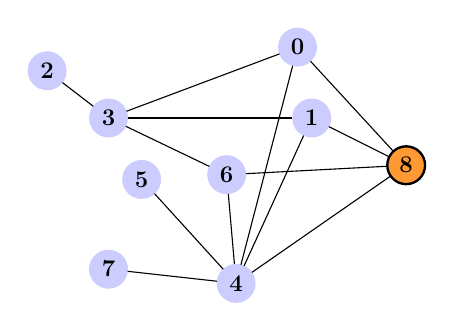
\begin{tikzpicture}[scale=0.6, transform shape,every node/.style={circle, draw, minimum size=8mm, font=\bfseries\Large}, 
                    every edge/.style={draw, thick=0.5mm}, 
                    node distance=1cm]
% Nodes
\node[fill=blue!20,draw=blue!20](0) at (0,0){0};
\node[fill=blue!20,draw=blue!20](1) at (0.3,-1.5){1};
\node[fill=blue!20,draw=blue!20](6) at (-1.5,-2.7){6};
\node[fill=blue!20,draw=blue!20](4) at (-1.3,-5){4};
\node[fill=orange!80,draw=black,line width=0.3mm](8) at (2.3,-2.5){8};
\node[fill=blue!20,draw=blue!20](3) at (-4,-1.5){3};
\node[fill=blue!20,draw=blue!20](5) at (-3.3,-2.8){5};
\node[fill=blue!20,draw=blue!20](2) at (-5.3,-0.5){2};
\node[fill=blue!20,draw=blue!20](7) at (-4,-4.7){7};

% % Edges
\draw (0) -- (8);
\draw (0) -- (4);
\draw (0) -- (3);
\draw (1) -- (3);
\draw (1) -- (8);
\draw (1) -- (4);
\draw (3) -- (6);
\draw (6) -- (8);
\draw (6) -- (4);
\draw (3) -- (2);
\draw (5) -- (4);
\draw (8) -- (4);
\draw (7) -- (4);

\end{tikzpicture}

    \caption{\small{Eight qubit graph state(blue) with one message qubit(orange).}}
    \label{fig:8 qubit cluster_8}
\end{figure}

\noindent Extension of this base graph code to the other BACs in the $[[n,1,3]]$ family is shown in Appendix \ref{APPENDIX: [[9,1,3]] code}.
We define the base code $\mathcal{B}_8$ as follows:
\begin{align}
g_1 &= X_0 X_1,\  g_2= X_2Z_3, \ g_3= Z_0 Z_1 Z_2 X_3 Z_6,\ g_7 = Z_4 X_7  \nonumber\\
g_4 &= Y_0 Z_1 Z_3 Y_4 Z_5Z_6 Z_7,\  g_5 = Z_4 X_5, 
\ g_6 = X_0X_6,
\label{eq:family_generators}
\end{align}

\noindent with logical operators
\[
Z_L = X_0 Z_3 Z_4, \qquad X_L = Z_0 Z_1Z_4Z_6.
\]


\noindent Its single-qubit error syndromes are shown in Table~\ref{tab:errors_due_to_faults_8}, with corresponding hook errors for the generators $g_3$ and $g_4$ in Table~\ref {tab:errors_due_to_faults_8_1}. 

\begin{table}[h]
\centering
\scriptsize
% \resizebox{0.4\textwidth}{!}{%
  % remove external padding so colored boxes touch vertical rules
  \setlength{\tabcolsep}{0pt} % IMPORTANT
  \renewcommand{\arraystretch}{1.2} % row height

  % Use simple centered columns; internal padding is handled by \PadCell / \PadCellColor
  \begin{tabular}{|c|c|c|c|}
    \hline
    \textbf{Data Error}  & \textbf{ Syndrome } & \textbf{ Data Error } & \textbf{ Syndrome } \\ \hline


    \rowcolor{gray!10}
    $Z_0$  & 1001010  & $Z_1$    &  1000000      \\ \hline
    $Z_2$  & 0100000  & $Z_3$    &  0010000      \\ \hline

    \rowcolor{gray!10}
    $Z_4$  & 0001000  & $Z_5$    &  0000100      \\ \hline
    $Z_6$  & 0000010  & $Z_7$    &  0000001      \\ \hline

    \rowcolor{gray!10}
    $X_0$    &  0011000      & $X_1$  & 0011000  \\ \hline 
    $X_2$    &  0010000      & $X_3$  & 0101000 \\ \hline

    \rowcolor{gray!10}
    $X_4$    & 0001101      & $X_5$  & 0001000    \\ \hline
    $X_6$    &  0011000     & $X_7$  & 0001000   \\ \hline

    \rowcolor{gray!10}
    $Y_0$  & 1010010  & $Y_1$    &  1011000      \\ \hline
    $Y_2$  & 0110000  & $Y_3$    &  0111000      \\ \hline
    

    \rowcolor{gray!10}
    $Y_4$  & 0000101  & $Y_5$    &  0001100     \\ \hline
    $Y_6$  & 0011010  & $Y_7$    &   0001001     \\ \hline

  \end{tabular}
% }
% }
\caption{Single-qubit error syndromes for the $[[8,1,3]]$ code}
\label{tab:errors_due_to_faults_8}
\end{table}



\begin{table}[h]
\centering
\scriptsize
% \resizebox{0.4\textwidth}{!}{%
  % remove external padding so colored boxes touch vertical rules
  \setlength{\tabcolsep}{0pt} % IMPORTANT
  \renewcommand{\arraystretch}{1.2} % row height

  % Use simple centered columns; internal padding is handled by \PadCell / \PadCellColor
  \begin{tabular}{|c|c|c|c|}
    \hline
    \textbf{ Data Error } & \textbf{ Syndrome } & \textbf{ Data Error } & \textbf{ Syndrome } \\ \hline

  
    \rowcolor{gray!20}
    \multicolumn{4}{|c|}{\boldmath\textbf{$Y_0 Z_1 Z_3 Y_4 Z_5 Z_6 Z_7$} $\longrightarrow$ $Z_1Y_4Y_0Z_5Z_3 Z_7Z_6$} \\ \hline

    % now rows; for yellow cells use \PadCellColor to ensure full coverage
    $Z_1X_4$  & 1001101  & $Z_1Y_4$    &  1000101      \\ \hline
    $Z_1YZ_4$  & 1001000  & $Z_1Y_4X_0$   &  1011101      \\ \hline
    $Z_1Y_4Y_0$  & 0010111  & $Z_1Y_4Z_0$    & 0001111      \\ \hline
    $Z_1Y_4Y_0X_5$  & 0011111  & $Z_1Y_4Y_0Y_5$    &  0011011      \\ \hline
    $Z_1Y_4Y_0Z_5$  & 0010011  & $Z_1Y_4Y_0Z_5X_3$    & 0111011      \\ \hline
    $Z_1Y_4Y_0Z_5Y_3$    &  0101011   & $Z_1Y_4Y_0Z_5Z_3$    &  0000011      \\ \hline
     $Z_1Y_4Y_0Z_5Z_3X_7$    &  0001011   & $Z_1Y_4Y_0Z_5Z_3Y_7$    &  0001010      \\ \hline

   



    
\rowcolor{gray!20}
    \multicolumn{4}{|c|}{\boldmath\textbf{$Z_0Z_1 Z_2 X_3Z_6$} $\longrightarrow$ $Z_0Z_2Z_1X_3Z_6$} \\ \hline

    % now rows; for yellow cells use \PadCellColor to ensure full coverage
   $Z_0X_2$  & 1011010  & $Z_0Y_2$    &  1111010      \\ \hline
   $Z_0Z_2$  & 1101010  & $Z_0Z_2X_1$    &  1110010      \\ \hline
   $Z_0Z_2Y_1$  & 0110010  & $Z_0Z_2Z_1$    &  0101010      \\ \hline
   $Z_0Z_2Z_1Y_3$  & 0010010  & $Z_0Z_2Z_1Z_3$    &  0111010      \\ \hline

  \end{tabular}

\caption{Propagated hook errors in the $[[8,1,3]]$ code with their syndromes for the corresponding stabilizers.
The rearranging of stabilizers is illustrated in grey boxes. 
}
\label{tab:errors_due_to_faults_8_1}
\end{table}


\noindent The family $\mathcal{B}_n$ for $n\ge 8$ is obtained by extending the stabilizer set with
\begin{align}
g_4^{(n)} &= Y_0 Z_1Z_3 Y_4 Z_5Z_6 Z_7 \prod_{j=8}^{n-1} Z_j, \nonumber\\
g_j &= Z_4 X_j, \qquad 8 \le j \le n-1.
\end{align}
We now show that this proposed extension to $[[n,1,3]]$ family preserves the stabilizer code properties.





\begin{lemma}
\label{lem:logical_commutation}
For every $n\ge 8$, the logical operators of the base code $\mathcal{B}_8$ commute with all the stabilizer generators of $\mathcal{B}_n$ and also satisfy the anticommutativity between the logical operators themselves.
Hence, $X_L$ and $Z_L$ define nontrivial logical operators of $\mathcal{B}_n$ of weight three.
\end{lemma}

\begin{proof}
The logical operators of the base code $\mathcal{B}_8$ is
\[
Z_L = X_0 Z_3 Z_4, \qquad X_L = Z_0 Z_1 Z_4Z_6
\]
The anti-commutation ($X_L Z_L=-Z_L X_L$) between these logicals is obvious.
Since the two operators overlap nontrivially on qubit $0$ and commute on all the other qubits.

\noindent We now check the commutation of the above logicals with the stabilizer generators for any codes from the $[[n,1,3]]$ family.
The generators of the base code $\mathcal{B}_8$ commute with $X_L$ and $Z_L$, as can be seen from Eq. \ref{eq:family_generators}. 
For $n>8$, the only additional generators to $\mathcal{B}_8$ are
\[
g_j = Z_4 X_j, \,\,\forall \,\, 8\le j\le n-1,
\]
and
\[
g_4^{(n)} = Y_0 Z_1Z_3 Y_4 Z_5Z_6 Z_7 \prod_{j=8}^{n-1} Z_j.
\]
\noindent Since $X_L$ and $Z_L$ have no support on qubits $j\ge 8$, both commute with every $g_j$. 
Further, the operator $Z_L=X_0Z_3Z_4$ anticommutes with $g_4^{(n)}$ on qubits $0$ and $4$; therefore, both operators commute overall. 
Similarly, $X_L=Z_0Z_1Z_4Z_6$ also anticommutes with $g_4^{(n)}$ on qubits $0$ and $4$, therefore overall these two also commutes.
Thus $X_L$ and $Z_L$ commute with all stabilizers of $\mathcal{B}_n$ for every $n\ge 8$.
\end{proof}

\begin{theorem}[Distance preservation]
\label{thm:distance}
If the base code $\mathcal{B}_8$ is a distance $d=3$ code, then all the codes $\mathcal{B}_n$ in the family are also distance $d = 3$ codes, generating a family of $[[n,1,3]]$ codes for all $n \ge 8$.
\end{theorem}

\begin{proof}
The proof of this theorem directly follows from Lemma \ref{lem:logical_commutation}.
The proposed family of codes encodes a single logical qubit, as discussed in the MBQC-based construction of graph codes. 
Using Lemma \ref{lem:logical_commutation} we know that $Z_L = X_0Z_3Z_4$ and $X_L = Z_0Z_1Z_4Z_6$ forms weight $3$ logical operators of $\mathcal{B}_n$.
% the operators $X_L$ and $Z_L$ belong to the normalizer of $\mathcal{S}_n$ and define logical operators of weight three. 
Hence $d(\mathcal{B}_n)\le 3$.\\\\
Now assume we have a logical operator $L_e=(x|z)\in N(\mathcal{S}_n)\setminus \mathcal{S}_n$ such that ${w}_{(L_e)}\le 2$.
Here $x,z$ are symplectic representations of an $n$-qubit Pauli operator.
To be a valid logical, this should commute with the newly proposed stabilizer $g_j = Z_4X_j: j\in\{5,7,8 \dots,n-1\}$ for any $\mathcal{B}_n$.
The commutativity implies that in the symplectic form, if $x_4=1$ for the logical, then $z_j=1$ for all $j\in\{5,7,8\dots,n-1\}$.
This directly implies that for a general $\mathcal{B}_n$,the logicals and the stabilizer mutually satisfy
\[
x_4 + z_j = 0 \ \text{mod}  \ 2.
\]

\noindent Therefore, for $n \geq 8$, the logical $L_e$ must atleast be supported on the qubit $5$ and $7$.
This suggests $w_{(L_e)}\ge 3$, which contradicts our initial assumption of having a logical operator of weight less equals $2$.\\
% Hence $x_4=0$ and $z_j=0$ for all such $j$.
\noindent Now we consider the case where $x_4 = 0$.
In this case, there are $3$ natural possibilities of a weight two logical operator, from which the only valid possibility is where the logical operator $L_e$ has only non-zero $x$ values in symplectic form, i.e., $z_j = 0 \,\,\forall\,\, j\in\{5,7,8\dots,n-1\}$.
The other possibilities, where $L_e$ has non-zero $z$ values directly anti-commute with atleast one of the stabilizers for $\mathcal{B}_n$.\\
Now, if $L_e$ has only non-zero $x$ values, then any remaining support of the logical operator on qubits $j\ge 8$ is either inconsistent because it violates the commutation with stabilizers or any stabilizer-equivalent operators, i.e.
\[
X_j X_k = g_j g_k, \quad X_j X_5 = g_j g_5, \quad X_j X_7 = g_j g_7.
\]
Thus $L_e$ reduces to an operator on qubits $\{0,\dots,7\}$.\\\\
\noindent Since $\mathcal{B}_8$ is a distance $3$ code, encoding a single logical qubit, there can be no other nontrivial logical operator of weight $\le 2$.
% so $E\in\mathcal{S}_n$, a contradiction. 
% Hence $d(\mathcal{C}_n)\ge 3$, and 
Hence, the only possibility that remains is that $d(\mathcal{B}_n)=3$.
\end{proof}
\noindent Now, as we have proved that the proposed family of codes $\mathcal{B}_n$ satisfies all the properties of a distance $d=3$ stabilizer code, we further show that these codes preserve the bare property of the base code $\mathcal{B}_8$.
\begin{theorem}[Preservation of the BAC property]
\label{thm:bare_recursion}
All the non-trivial hook errors generated due to the errors propagated from the generator $g_3$ and newly introduced stabilizer $g_4^{(n)}$ of the code $\mathcal{B}_n$ can always be assigned to unique syndromes.

\end{theorem}
\begin{proof}
We have already discussed that the base code $\mathcal{B}_8$ supports unique syndromes for each of the non-trivial hook errors generated from its stabilizer set (refer to Table~\ref{tab:errors_due_to_faults_8} and Table~\ref{tab:errors_due_to_faults_8_1}).
We consider the syndrome uniqueness of the stabilizers $\Sigma_n^{(4)}$ and $g_3$ because any other stabilizer of $\mathcal{B}_n$ has always weight $2$, therefore they do not produce a non-trivial hook error.
Now let us denote $\Sigma_n^{(4)}$ as the set of possible syndromes generated due to the propagation of hook-errors from the ordered measurement of the stabilizer $g_4^{(n)} = Z_1\, Y_4\, Y_0\, Z_5\, Z_3\, Z_7\, Z_6\, Z_8\cdots Z_{n-1}$ and $\Sigma_n^{(3)}$ denote the corresponding set arising from the ordered measurement of $g_3 = Z_0\, Z_2\, Z_1\, X_3\, Z_6$.
In Appendix \ref{APPENDIX: [[9,1,3]] code}, we show that for $\mathcal{B}_9$ and $\mathcal{B}_{10}$ all syndromes in $\Sigma_n^{(4)}\cup\Sigma_n^{(3)}$ are non-zero, pairwise distinct within each set, and distinct across the two sets.
Now, for $n \geq 10$, under the extension $\mathcal{B}_n\to\mathcal{B}_{n+1}$, all previously existing propagated hook errors retain their original syndrome on the first $n-1$ coordinates, since the measurement circuits are unchanged except for the appended interaction on qubit $n$.\\\\
Now, this extension introduces a new stabilizer generator $ g_n = Z_4 X_n$, which contributes an additional syndrome bit. 
For every previously existing propagated hook errors due to the faults from the measurement circuit of $g_4^{(n)}$, commutation with $g_n$ yields an additional syndrome bit equal to $1$.
This imply 
\[
\Sigma_{n+1}^{(4)} = \{(s,1): s\in \Sigma_n^{(4)}\}\cup\{\eta_{n+1}\},
\]
where \[\{\eta_{n+1} = Z_1\, Y_4\, Y_0\, Z_5\, Z_3\, Z_7\, Z_6\, Z_8\cdots P_{n-1}, \  \ P = \{X, Y\}\}\] is the set of syndromes of the newly introduced longest suffix hook error due to appended factor $Z_n$ in $g_4^{(n+1)}$. 
\noindent On the other hand, the propagated hook errors arising from $g_3$ have no support on qubits $4$ and $n$.
Therefore, all those hook errors commute with $g_3$, which implies
\[
\Sigma_{n+1}^{(3)} = \{(s,0): s\in \Sigma_n^{(3)}\},
\]
Hence, the two set of syndromes assigned to each of the non-trivial hook errors due to the stabilizers $g_4^{(n)}$ and $g_3$ remains disjoint.\\\\
For $n\ge 11$, additional correlated propagated errors may produce syndrome collisions within the $g_4^{(n)}$ sector. However, these collisions occur only between stabilizer-equivalent errors. 
Indeed, in the first nontrivial case $n=11$,
\[
E_1=Z_1Y_4Y_0Z_5Z_3Z_7Z_6Z_8Y_9,\] and \[
E_2=Z_1Y_4Y_0Z_5Z_3Z_7Z_6Z_8Z_9X_{10}
\]
have identical syndromes, while
\[
E_1E_2 = X_9X_{10}=(Z_4X_9)(Z_4X_{10})\in\mathcal S_{11}.
\]
More generally, every new correlated propagated error arises by replacing a terminal factor $Y_j$ with $Z_jX_{j+1}$, and the corresponding pair of errors differs by
\[
X_jX_{j+1}=(Z_4X_j)(Z_4X_{j+1})\in\mathcal S_{n+1}.
\]
Thus, all such collisions lie within a single stabilizer coset.\\\\
\noindent Therefore, all newly introduced propagated errors are either assigned distinct syndromes or are stabilizer-equivalent to previously assigned error classes. In both cases, the code's bare property is preserved. 
Hence, we can assign unique syndromes to all such non-trivial errors, and the lookup-table decoder extends consistently under $\mathcal{B}_n\to\mathcal{B}_{n+1}$.

\end{proof}
\section{Experimental setup}
\label{sec:experimental setup}
% %\vspace{-0.3cm}
\noindent In this section, we validate the performance of the BACs obtained from graph codes.
We perform numerical error rate simulations on the BAC codes and the flag method used for the respective graph codes.
The goal is to compare the performance of BACs with the flag qubit-based method of fault tolerance against hook errors.
Error-rate simulations demonstrate how ancilla-induced hook errors affect logical error rates for the $[[n,1,3]]$ BACs.
We use a lookup table decoder to justify the optimal performance achievable by the BACs. 
We estimate the logical error rates of given QECCs using CHP (CNOT-Hadamard-Phase) stabilizer simulator~\cite{PhysRevA.70.052328}.\\
The general simulation framework involves an error-correction cycle with random noise, followed by a final noise-free error-correction round.
The noise model is described later in this section.
% Each trial consists of an initial error correction under random noise, followed by a final noise-free correction using a look-up decoder.
In both rounds, the ancillary qubits used for syndrome extraction undergo a reset before the start of the error-correction round.
% repeated up to two times with freshly prepared ancillary qubits. 
Further, we construct the look-up table for decoding in three parts.
First, we include syndromes obtained from the parity check matrix $\mathbf{H_\mathrm{xyz}}$.
Next, we add the syndromes that arise from the hook errors propagated during the error correction cycle.
Finally, the remaining unmatched syndromes are assigned to its correspoinding minimum-weight Pauli operators using the parity-check matrix 
\subsection{Error rate calculation}
\noindent We perform $10^8$ trials of Monte Carlo simulations and estimate the logical error rates for each physical error probability.
After FT error-correction rounds and perfect decoding using a lookup table, each trial is classified according to the residual operator acting on the data qubits.
A trial contributes to a logical error if the residual nontrivial operator anti-commutes with one of the logical operators and commutes with all the stabilizer operators. 
We obtain the error rates from the ratio of the respective error-prone trial counts to the total number of trials.
\subsection{Noise Models}
\noindent We perform the numerical experiments under two noise models, standard depolarizing noise and anisotropic noise.
\subsubsection{Standard Depolarizing Noise Model}
\noindent The standard depolarizing noise model assumes a symmetric depolarization error after each quantum gate with a probability $p$.
This produces a maximally mixed state $I/2$, with probability $p$, and the quantum state remains unchanged with probability of $1-p$.
This noise model can also be described in terms of discrete Pauli errors and reflects one of the most standard circuit-level noise models.
\begin{itemize}
    \item \textbf{Single-qubit gate errors:} After each single-qubit gate a Pauli error ($\{X, Y, Z\}$) occurs with probability $p_{s}/3$. 
    \item \textbf{Two-qubit gate errors:} After each two-qubit gate, the corresponding qubits can suffer error from $\{I, X, Y, Z\}\otimes \{I, X, Y, Z\}\backslash\{I\otimes I\}$.
    Each of the possible errors occurs with probability $p_t/15$.
    \item \textbf{Measurement errors:}
    Each measurement outcome is followed by a bit flip error with probability $p_{m}$.
     \item \textbf{State preparation errors:} The initial states prepared in $\ket{0}$ flips to $\ket{1}$ and the state prepared in $\ket{+}$ flips to $\ket{-}$ with probability $p_{p}$.
\end{itemize}
\subsubsection{Anisotropic Noise Model}
%\vspace{-0.2cm}
\noindent The anisotropic noise model is conditioned on the assumption that a two-qubit error will always align with the target operation.
It considers the effects of the under- or over-rotation of the gates in the ion trap qubits~\cite{parrado2020crosstalk,PhysRevLett.82.1971}.
The effects of this noise model can also be described in terms of the discrete Pauli errors.
\begin{itemize}
    \item \textbf{Single-qubit errors, measurement/ readout errors, and state preparation errors}: These errors are applied with probabilities $p_s$, $p_{m}$, and $p_{p}$ respectively and have the same effect as described in the standard depolarizing noise model.
    \item \textbf{Two-qubit gate errors:} 
    Each two-qubit gate controlled-P (CP) is followed by a $Z \otimes P$ error with probability $p_t$.
    Also, the corresponding quibits suffer from a single qubit depolarizing error with probability $p_s$. 
    \end{itemize}
% %\vspace{-0.1cm}
\noindent We now analyze various $[[n,1,3]]$ BACs and flag qubit method under this experimental setup.
For simplicity, we consider $p_m = p_p = p_s$.
\section{Results}
\label{sec:results analysis}
\noindent The numerical simulations we perform yield a logical error rate vs physical error rate plot for each $[[n,1,3]]$ code.
We perform error-rate simulations for both the BACs from our work and the flag-based error-correction method on the same graph codes.
These error rate simulations are used to extract the pseudo-thresholds for each code.
In Figure \ref{fig:flag_bare_bp_comparison} and Figure \ref{fig:bare_flag_ani_comparison}, we plot the logical error rates obtained for the BACs and flag method for the depolarizing and anisotropic noise, respectively.

\begin{figure}[htbp]
    \centering  
    
    \includegraphics[width=0.45\textwidth]{bac-ler-dp.png} 
    \includegraphics[width=0.45\textwidth]{flag-ler-dp.png} 
    
    \caption{We show the logical error rate vs physical error rate plots of the $[[n,1,3]]$ QECCs under the standard depolarizing noise model.
    The first figure shows the logical error rates for the BAC method of FT syndrome extraction, and the latter shows the same for the flag qubit-based FT syndrome extraction.
    We also note the pseudo-thresholds of each QECC for these different FT methods.
    } 
    
    \label{fig:flag_bare_bp_comparison} 
\end{figure}
\begin{figure}[htbp]
    \centering  
    
    \includegraphics[width=0.45\textwidth]{bare-ler-ani.png} 
    % \\
    \includegraphics[width=0.45\textwidth]{flag-ler-ani.png}
    
    \caption{We show the logical error rate vs physical error rate plots of the $[[n,1,3]]$ QECCs under the anisotropic noise model.
    The first figure shows the logical error rates for the BAC method of FT syndrome extraction, and the latter shows the same for the flag qubit-based FT syndrome extraction.
    We also note the pseudo-thresholds of each QECC for these different FT methods.
    } 
    
    \label{fig:bare_flag_ani_comparison} 
\end{figure}
\noindent We also show the pseudo-threshold comparisons for the $[[n,1,3]]$ QECCs with both bare and flag methods under the two different noise models, as shown in Figure \ref{fig:flag_ani_comparison}.
We observe that the $[[6,1,3]]$ BAC offers no pseudo-threshold for the standard depolarizing noise model.
This phenomenon upholds the fact that the $[[6,1,3]]$ graph code does not have enough syndrome space to support the correlated hook error corrections.
A detailed analysis of the $[[6,1,3]]$ graph code is discussed in Appendix \ref{APPENDIX: [[6,1,3]] code}.
Although we observe a non-zero pseudo-threshold for the $[[6,1,3]]$ BAC under the anisotropic noise model.
To the best of our knowledge, this code has the most optimized code rate, which shows asymptotic fault tolerance under the anisotropic noise model.\\\\
Further, among the simulated QECCs, the $[[7,1,3]]$ and $[[12,1,3]]$ codes perform better than the others in both the bare and flag methods, as shown in the error rate simulation plots.
A key observation from the extracted pseudo-thresholds for the two fault-tolerant methods is that the bare method either outperforms or performs similarly to the flag-based method.
The error-correction capability is evident from the fact that the bare method yields a pseudo-threshold for depolarizing noise that is almost the same as the flag method's from $[[7,1,3]]$ onwards.
Whereas under anisotropic noise model, BAC performs almost equal to or better than the flag qubit method from $[[6,1,3]]$ onwards.



% \begin{figure}[t]
%     \centering  
    
%     \includegraphics[width=0.45\textwidth]{new_imgs/threshold-comp-dp.png} 
%     % \\
%     % \includegraphics[width=0.45\textwidth]{new_imgs/threshold-comp-ani.png} 
    
%     \caption{Comparison of Pseudo-thresholds for different $[[n,1,3]]$ QECCs for both the bare and flag fault-tolerant method under the deplorizing and anisotropic noise.} 
    
%     \label{fig:flag_ani_comparison} 
% \end{figure}




\begin{figure}[h]
\centering

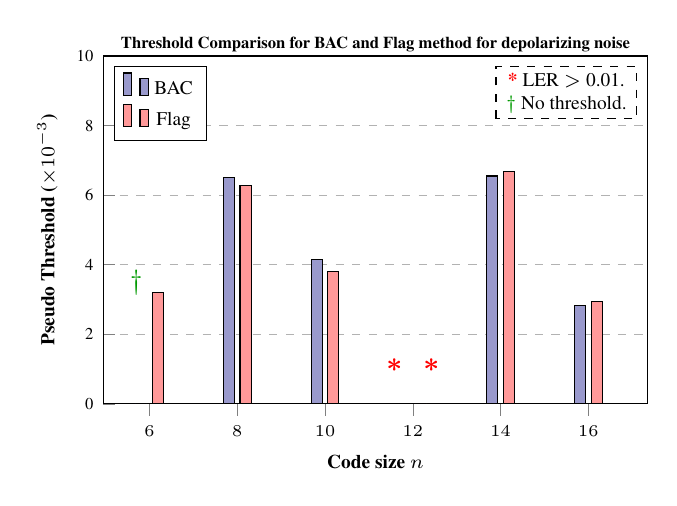
\begin{tikzpicture}

\begin{axis}[
    xtick pos=left,
    ytick pos=left,
    ybar,
    bar width=4pt,
    width=8.5cm,
    height=6cm,
    ymin=0,
    ymax=0.01,
    xtick={6,8,10,12,14,16},
    xmin=5.8,
    xmax=16.5,
    enlarge x limits=0.08,
    scaled y ticks=false,
    ytick={0,0.002,0.004,0.006,0.008,0.010},
    yticklabels={0,2,4,6,8,10},
    yticklabel style={font=\fontfamily{ptm}\fontsize{6}{7}\selectfont},
    ylabel={\textbf{\scriptsize Pseudo Threshold ($\times 10^{-3}$)}},
    xlabel={\textbf{\scriptsize Code size $n$}},
    title={\textbf{Threshold Comparison for BAC and Flag method for depolarizing noise}},
    title style={font=\fontfamily{ptm}\fontsize{6}{7}\selectfont\bfseries,yshift=-8pt},
    xticklabel style={font=\fontfamily{ptm}\fontsize{6}{7}\selectfont},
    ylabel style={font=\fontfamily{ptm}\fontsize{7}{9}\selectfont},
    xlabel style={font=\fontfamily{ptm}\fontsize{7}{9}\selectfont},
    ymajorgrids=true,
    grid style={dashed, gray!60},
    legend style={
        at={(0.02,0.97)},
        anchor=north west,
        font=\fontfamily{ptm}\fontsize{6}{7}\selectfont,
        draw=black,
        fill=white
    }
]
 \node at (axis cs:15.5,0.0093)
        {
   \fontfamily{ptm}\fontsize{7}{8}\selectfont
    \color{red} \textbf{*}  \textcolor{black}{LER $>$ 0.01.}
            };
\node at (axis cs:15.5,0.0086)
        {
   \fontfamily{ptm}\fontsize{7}{8}\selectfont
   \color{green!60!black}$\dagger$ \color{black} No threshold.
            };

          
\node at (axis cs:12,0.001)
        { \bfseries
     \color{red}* \ *          };

\node at (axis cs:5.7,0.0035)
        {\fontfamily{ptm}\fontsize{10}{12}\selectfont\bfseries 
    \color{green!60!black} $\dagger$      };
\addplot[
    fill=blue!50!black!40,
    draw=black
]
coordinates {
    (6,0.00)
    (8,0.006506579)
    (10,0.004155588)
    (12,0.00)
    (14,0.006548138)
    (16,0.002836444)
};

\addplot[
    fill=red!40!white,
    draw=black
]
coordinates {
    (6,0.003195418)
    (8,0.006277374)
    (10,0.00379584)
    (12,0)
    (14,0.006679473)
    (16,0.002949541)
};
%   coordinates {
%     (11,0.0010)
%     (15,0.005)
% };

\draw[dashed,
    line width=0.5pt]
(axis cs:13.9,0.0082)
rectangle
(axis cs:17.1,0.0097);
  
  
  
  % \draw[dotted,thick] (axis cs:8,0.001) rectangle(axis cs:12,0.006);
\legend{
    \scriptsize BAC,
    \scriptsize Flag 
}

ll\end{axis}

\end{tikzpicture}

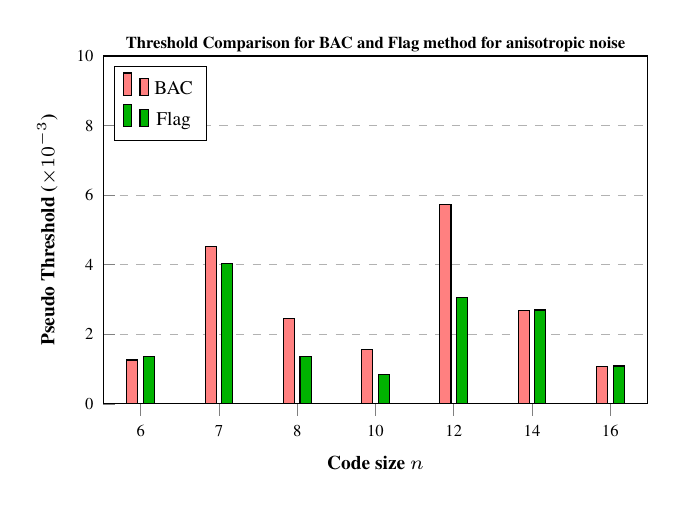
\begin{tikzpicture}

\begin{axis}[
    xtick pos=left,
    ytick pos=left,
    ybar,
    bar width=4pt,
    width=8.5cm,
    height=6cm,
    ymin=0,
    ymax=0.01,
    symbolic x coords={6,7,8,10,12,14,16},
    xtick=data,
    enlarge x limits=0.08,
    scaled y ticks=false,
    ytick={0,0.002,0.004,0.006,0.008,0.010},
    yticklabels={0,2,4,6,8,10},
    yticklabel style={font=\fontfamily{ptm}\fontsize{6}{7}\selectfont},
    ylabel={\textbf{\scriptsize Pseudo Threshold ($\times 10^{-3}$)}},
    xlabel={\textbf{\scriptsize Code size $n$}},
    title={\textbf{Threshold Comparison for BAC and Flag method for anisotropic noise}},
    title style={font=\fontfamily{ptm}\fontsize{6}{7}\selectfont\bfseries,yshift=-8pt},
    xticklabel style={font=\fontfamily{ptm}\fontsize{6}{7}\selectfont},
    ylabel style={font=\fontfamily{ptm}\fontsize{7}{9}\selectfont},
    xlabel style={font=\fontfamily{ptm}\fontsize{7}{9}\selectfont},
    ymajorgrids=true,
    grid style={dashed, gray!60},
    legend style={
        at={(0.02,0.97)},
        anchor=north west,
        font=\fontfamily{ptm}\fontsize{6}{7}\selectfont,
        draw=black,
        fill=white
    },
]




% \node at (0.5,0.95){* No threshold for $[[613]]$};
% BAC
\addplot[
    fill=red!50,
    draw=black
]
coordinates {
    (6,0.001259491)
    (7,0.00453067)
    (8,0.002455143)
    (10,0.001565204)
    (12,0.005717529)
    (14,0.002689754)
    (16,0.001076653)
};
% FLAG
\addplot[
    fill=black!30!green,
    draw=black
]
coordinates {
    (6,0.001355485)
    (7,0.004047141)
    (8,0.001357602)
    (10,0.0008493999)
    (12,0.003064659)
    (14,0.002697604)
    (16,0.001089010)
};

\legend{
    \scriptsize BAC,
    \scriptsize Flag 
}
\end{axis}

\end{tikzpicture}

\caption{Comparison of Pseudo-thresholds for different $[[n,1,3]]$ QECCs for both the bare and flag fault-tolerant method under the depolarizing and anisotropic noise.}
\label{fig:flag_ani_comparison}
\end{figure}





\section{Conclusion}
\label{sec:conclusion}

\noindent In this work, we have constructed and analyzed the fault tolerance of a family of $[[n,1,3]]$ non-CSS QECCs using graph codes. 
We demonstrate error resilience against hook errors using a single ancilla qubit for syndrome measurement and proposed a class of $[[n,1,3]]$ bare ancilla codes, which we obtain using a base graph code $\mathcal{B}_8$.
We analytically showed the validity of the distance $3$ stabilizer QECCs $[[n,1,3]]$ and further established the BAC properties of the codes in this family.
In summary, this demonstration sheds light on how FT codes can be found from graph codes.
Using this framework, we are able to find the most optimized (in terms of code rate) BAC, namely the $[[6,1,3]]$ code, which has a non-zero pseudo threshold under the anisotropic noise model.\\\\
There exist many open directions following from this work. 
Extending these constructions to longer distances or to multiple logical qubit codes would test the universality of our frameworks. 
Since all the codes considered here arise from graph code constructions, further exploration of the interplay between graph structures and FT properties could yield new insights into the connections between bare-ancilla and graph codes. 
% \section{Data Availability}
% The data and codes used for the numerical experiments are available from the authors on reasonable requests.
\begin{acknowledgments}
\noindent The authors thank Rahul Garg for his assistance with the proofs and Pranav Maheshwari for his valuable suggestions in preparing this manuscript.
R.J. acknowledges funding support from the Department of Science and Technology Grant No. DST/QTC/NQM/QComm/2024/2. 
H.G. and M.B. thank IISER Bhopal for providing the necessary computational resources and the institute fellowship that supports their doctoral work.
\end{acknowledgments}

% \bibliographystyle{apsrev4-2} % use APS reference style
\bibliography{apssamp}% Produces the bibliography via BibTeX.
\newpage
\appendix

\section{MBQC Encoding }
\label{APPENDIX: MBQC min distance}
\noindent A  graph state can be mathematically represented as an undirected graph $G = (V, E)$, where $V$  denotes the set of vertices corresponding to the qubits, and $ E$  represents the edges corresponding to $\mathrm{CZ}$ gates between the qubits.
And all the $\mathrm{CZ}$ gates connected with a vertex $i$ can be written as:
\begin{equation}
    \prod_{(i,j)\in E_i}\mathrm{CZ}_{ji} = \prod_{j\in \mathcal{N}_i} I_j \otimes \ket{0}\bra{0}_i + \prod_{j\in \mathcal{N}_i}Z_j\otimes \ket{1}\bra{1}_i
    \label{cz equation}
\end{equation}
where $E_i$ represents the set of all edges connected to node $i$ and $\mathcal{N}_i$ the set of all neighboring nodes of node $ i \in V$.

\begin{proof}
Consider a state $\ket{\psi_m}$, an $n$-qubit cluster with one message qubit $i.e.$  $\ket{\phi_{m}} = \alpha\ket{0}_{m} + \beta\ket{1}_{m}$, where m = n+1. 

\begin{equation*}
\begin{split}
    \ket{\psi_m} = \ & \prod_{i \in \{1,2,\cdots,n\}} \prod_{ \substack{(i,j) \in E_i \\ j>i }}\mathrm{CZ}_{ij} \left ( \ket{+}^{\otimes n}\ket{\phi_{m}}\right ) \\
     = \ &  \Biggl ( \prod_{i \in \{1,2,\cdots,n\}} \prod_{ \substack{(i,j) \in E_i\setminus	E_m \\  j>i }}\mathrm{CZ}_{ij}  \ \biggl( \\  & \prod_{\substack{(m,k)\in E_{m} \\ k \in (1,2,\cdots ,n)}}\mathrm{CZ}_{mk} \left ( \ket{+}^{\otimes n} \ket{\phi_{m}}\right ) \biggl )\Biggl ) \\
     \ & \text{where $E_{m}$ represents the set of all the edges} \\ & \text{connected to the message qubit and using} \\ & \text{Eq.\eqref{cz equation}, we get}\\
     = \ &  \left ( \prod_{i \in \{1,2,\cdots,n\}} \prod_{ \substack{(i,j) \in E_i\setminus	E_m \\  j>i }}\mathrm{CZ}_{ij}\right)  \Biggr [ \biggl (  
    \prod_{k\in \mathcal{N}_{m}} \\ & I_k \otimes \ket{0}\bra{0}_{m}+\prod_{k\in \mathcal{N}_{m}}Z_k \otimes \ket{1}\bra{1}_{m} \biggl )  \ket{+}^{\otimes n}\ket{\phi_{m}}\Biggr ] \\
    = \ &  \left ( \prod_{i \in \{1,2,\cdots,n\}} \prod_{ \substack{(i,j) \in E_i\setminus	E_m \\  j>i }}\mathrm{CZ}_{ij}\right)  \Biggr[  \alpha  \ket{+}^{\otimes n} \ket{0}_{m}  +  \\ & \beta \prod_{k\in \mathcal{N}_{m}}Z_k   \ket{+}^{\otimes n} \ket{1}_{m}\Biggr] \\
    = \ & \alpha \mathrm{U} \ket{+}^{\otimes n }  \ket{0}_{m} +  \beta \mathrm{U}  \prod_{k\in \mathcal{N}_{m}}Z_k \ket{+}^{\otimes n} \ket{1}_{m}, \\ &  \text{where } \mathrm{U}  = \prod_{i \in \{1,2,\cdots,n\}} \prod_{ \substack{(i,j) \in E_i\setminus	E_m \\  j>i }}\mathrm{CZ}_{ij}. \\
    = \ & \alpha \ket{G}  \ket{0}_{m} +  \beta  \prod_{k\in \mathcal{N}_{m}}Z_k \ket{G}\ket{1}_{m}, \\ & \text{where} \ket{G} = \mathrm{U} \ket{+}^{\otimes n }.
\end{split}
\end{equation*}
Hence 
\begin{equation*}
\begin{split}
    \ket{\psi}=\ & \biggl( \alpha \ket{G} + \beta\prod_{k\in \mathcal{N}_{m}}Z_k\ket{G} \biggl) \dfrac{\ket{+}_m}{2} \quad + \\ &\biggl( \alpha \ket{G} - \beta\prod_{k\in \mathcal{N}_{m}}Z_k\ket{G} \biggl) \dfrac{\ket{-}_m}{2}.
\end{split}
\end{equation*}
\noindent After the measurement of the message qubit in a $X$ basis we will get the encoded state in  $\alpha \ket{G} + (-1)^{p}\beta\prod_{k\in \mathcal{N}_{m}}Z_k\ket{G} $ form, where $p$ will be mapped to 0  and 1 for the outcomes  $\ket{+}_{m}$ and $\ket{-}_{m}$ respectively. 
\end{proof}
%\vspace{-0.5cm}

\section{Bare code construction algorithm}
\label{APPENDIX: Bare code construction algorithm}
\noindent The Algorithm \ref{algo: bare code construction} checks each stabilizer generator separately.
It tells you which orderings $g_{j,\pi}$ are locally valid.
The below algorithm, $i.e$ Algorithm \ref{algo: global BAC construction}, then checks whether these local choices are mutually compatible at the level of the full code.

{\linespread{1}\selectfont
\begin{algorithm}[H]
\DontPrintSemicolon
\caption{Global construction of \texorpdfstring{$[[n,1,3]]$}{[[n,1,3]]} BACs}
\label{algo: global BAC construction}

\KwIn{
Modified parity-check matrix 
$\mathbf{H}_{\mathrm{xyz}}=[\mathbf{H}_\mathrm{x}|
\mathbf{H}_\mathrm{z}|
\mathbf{H}_\mathrm{x}\oplus\mathbf{H}_\mathrm{z}]$;\;
candidate lists 
$\mathcal{C}_j=\{(\tilde g_{j,\pi},
\mu^{j,\pi}_\mathtt{o},
\mu^{j,\pi}_\mathtt{a})\}$ 
obtained from Algorithm~\ref{algo: bare code construction}, 
for $j=1,\ldots,m$;\;

}

\KwOut{
List $\mathcal{B}_{ac}$ of valid BACs 
$(\mathcal{S}_{\mathrm{BAC}},\Pi,\Omega_{\mathrm{BAC}})$.
}

\BlankLine

Initialize $\mathcal{B}_{ac}\gets\emptyset$\;

$\Omega_{\mathrm{init}}\gets
\{\mathtt{syn}(E): E\in\{X_i,Y_i,Z_i\}_{i=1}^{n},
\mathtt{syn}(E)\neq 0\}$\;

\BlankLine

\SetKwFunction{Search}{Search}
\SetKwProg{Fn}{Procedure}{:}{}

\Fn{\Search{$j,\mathcal{S},\Pi,\Omega$}}{

    \If{$j=m+1$}{
        \If{
        $\operatorname{rank}_{\mathbb{F}_2}(\mathcal{S})=n-1$
        }{
            $\mathcal{B}_{ac}\gets
            \mathcal{B}_{ac}\cup\{(\mathcal{S},\Pi,\Omega)\}$\;
        }
        \Return\;
    }

    \ForEach{
    $C_{g_{j,\pi}}=(\tilde g_{j,\pi},
    \mu^{j,\pi}_\mathtt{o},
    \mu^{j,\pi}_\mathtt{a})
    $
    }{

        $h\gets\operatorname{op}(\tilde g_{j,\pi})$\;
        \tcp{$h$ is the Pauli operator corresponding to the ordered generator $\tilde g_{j,\pi}$.}

        $\Delta_c\gets
        \{\delta:
        (Q,\delta)\in
        \mu^{j,\pi}_\mathtt{a}\}$\;
        \tcp{$\Delta_c$ is the syndrome set of the correlated hook errors for $g_{j, \pi}$.}
        \If{$\Delta_c\cap\Omega\neq\emptyset$}{
            \textbf{continue}\;
        }
        \If{
        $\operatorname{rank}_{\mathbb{F}_2}
        (\mathcal{S}\cup\{h\})
        <
        \operatorname{rank}_{\mathbb{F}_2}(\mathcal{S})+1$
        }{
            \textbf{continue}\;
        }

        $\mathcal{S}'\gets\mathcal{S}\cup\{h\}$\;
        $\Pi'\gets
        \Pi\cup
        \{(\tilde g_{j,\pi},
        \mu^{j,\pi}_\mathtt{o},
        \mu^{j,\pi}_\mathtt{a})\}$\;
        $\Omega'_{}\gets\Omega\cup\Delta_c$\;

        \Search{$j+1,\mathcal{S}',\Pi',\Omega'$}\;
    }
}

\BlankLine

\Search{$1,\emptyset,\emptyset,\Omega_{\mathrm{init}}$}\;

\Return $\mathcal{B}_{ac}$\;

\end{algorithm}
}
\noindent The set  $\Omega_{init}$ contains the syndromes already occupied by single-qubit data errors.
This is included because a valid distance-three BAC should not allow a hook-error syndrome to collide with a syndrome already assigned to a correctable single-qubit error.
The set $\Delta_c$ contains all correlated hook-error syndromes associated with one candidate ordered generator.
The condition $\Delta_c \cap \Omega = \emptyset$ ensures that no newly introduced hook-error syndrome collides with any syndrome already used by previously selected generators.
Finally, the rank test ensures that each accepted generator is independent of the previously selected generators.
Note that, for BACs designed to correct uncorrelated errors, the set $\Delta_c$ is constructed using $\mu^{j,\pi}_\mathtt{o}$ instead of $\mu^{j,\pi}_\mathtt{a}$.
\section{\texorpdfstring{$[[6,1,3]]$}{[[6,1,3]]} Bare ancilla code construction}
\label{APPENDIX: [[6,1,3]] code}
\noindent For the construction of the $[[6,1,3]]$ bare code, we first consider a six-qubit graph state with one message qubit. The message qubit is also connected with $\mathrm{CZ}$ gates.  
Hence, the first six qubits, namely those labeled 0 through 5, are prepared in the $\ket{+}$ state, and the seventh qubit, labeled 6, is the message qubit as seen in Figure \ref{fig:7 qubit cluster}.
\begin{figure}[h]
    \centering
    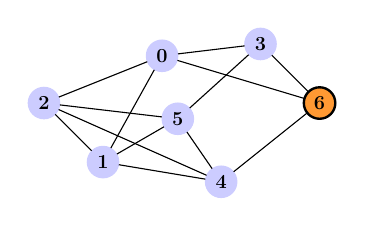
\begin{tikzpicture}[scale=0.5, transform shape,every node/.style={circle, draw, minimum size=8mm, font=\bfseries\Large}, 
                    every edge/.style={draw, thick=0.5mm}, 
                    node distance=1cm]
% Nodes
\node[fill=blue!20,draw=blue!20] (0) at (0, 1.2) {0};
\node[fill=blue!20,draw=blue!20] (1) at (-1.5, -1.5) {1};
\node[fill=blue!20,draw=blue!20] (2) at (-3, 0) {2};
\node[fill=blue!20,draw=blue!20] (3) at (2.5, 1.5) {3};
\node[fill=blue!20,draw=blue!20] (4) at (1.5, -2) {4};
\node[fill=blue!20,draw=blue!20] (5) at (0.4, -0.4) {5};
\node[fill=orange!80,draw=black,line width=0.3mm] (6) at (4, 0) {6};

% Edges
\draw (0) -- (1);
\draw (0) -- (2);
\draw (0) -- (3);
\draw (0) -- (6);
\draw (1) -- (2);
\draw (1) -- (4);
\draw (1) -- (5);
\draw (2) -- (4);
\draw (2) -- (5);
\draw (3) -- (5);
\draw (3) -- (6);
\draw (4) -- (5);
\draw (4) -- (6);


\end{tikzpicture}

    \caption{\small{Six qubit graph state with one message qubit(orange) which is measured in the $X$ basis.}}
    \label{fig:7 qubit cluster}
\end{figure}

\noindent We use Algorithm~\ref{algo: matrix method} to show the changes in the parity check matrix once the message qubit is measured in the $X$ basis. 
Consider the parity check matrix ($\mathbf{H}$ = [$\mathbf{H}_\mathrm{x}|\mathbf{H}_\mathrm{z}$]) of the graph state:
\begin{equation}
 \hat{\mathbf{H}}_6=\begin{bmatrix}
\scriptsize\begin{array}{c@{\hskip 7pt}c@{\hskip 7pt}c@{\hskip 7pt}c@{\hskip 7pt}c@{\hskip 7pt}c@{\hskip 7pt}c|c@{\hskip 7pt}c@{\hskip 7pt}c@{\hskip 7pt}c@{\hskip 7pt}c@{\hskip 7pt}c@{\hskip 7pt}c}
     1&0&0&0&0&0&0 &0&1&1&1&0&0&1  \\
     0&1&0&0&0&0&0 &1&0&1&0&1&1&0 \\
     0&0&1&0&0&0&0 &1&1&0&0&1&1&0 \\
     0&0&0&1&0&0&0 &1&0&0&0&0&1&1 \\
     0&0&0&0&1&0&0 &0&1&1&0&0&1&1 \\
     0&0&0&0&0&1&0 &0&1&1&1&1&0&0 
\end{array}\end{bmatrix}.
\label{matrix:before meas}
\end{equation}
First row of the above matrix corresponds to the first stabilizer $ X_0Z_1Z_2Z_3Z_6$ of the set $\mathcal{\hat{S}}_6$. 
This row is added with other rows corresponding to other stabilizers of the set $\mathcal{\hat{S}}_6$ so that all the stabilizers commute with $X_6$ except $ X_0Z_1Z_2Z_3Z_6$.
We remove the seventh, fourteenth column, and the first row from the matrix $ \hat{\mathbf{H}}_6$ because the message qubit is measured.
Operations and the changes are mentioned below in Eq.\eqref{eq: matrix after measurement}:
\begin{equation}  \scriptsize
\begin{split}
 & 
\begin{bmatrix}
\begin{array}{ccccccc|ccccccc}
    \tikz[remember picture]\node[inner sep=0pt] (a1) {1};&0&0&0&0&0&\tikz[remember picture]\node[inner sep=0pt] (a2){0}; &0&1&1&1&0&0&\tikz[remember picture]\node[inner sep=0pt] (a) {1}; \\
    0&1&0&0&0&0&0 &1&0&1&0&1&1& \tikz[remember picture]\node[inner sep=0pt] (b) {0}; \\ 
    0&0&1&0&0&0&0 &1&1&0&0&1&1& \tikz[remember picture]\node[inner sep=0pt] (c) {0}; \\
    1&0&0&1&0&0&0 &1&0&0&0&0&1&\tikz[remember picture]\node[inner sep=0pt] (d) {0}; \\
    1&0&0&0&1&0&0 &0&1&1&0&0&1&\tikz[remember picture]\node[inner sep=0pt] (e2) {0}; \\
   0&0&0&0&0&1& \tikz[remember picture]\node[inner sep=0pt] (a3){0}; 
   &0&1&1&1&1&0&\tikz[remember picture]\node[inner sep=0pt] (e) {0}; 
\end{array}
\end{bmatrix} \\ & \implies 
\mathbf{H}_6 =
\begin{bmatrix}
\begin{array}{c@{\hskip 7pt}c@{\hskip 7pt}c@{\hskip 7pt}c@{\hskip 7pt}c@{\hskip 7pt}c|c@{\hskip 7pt}c@{\hskip 7pt}c@{\hskip 7pt}c@{\hskip 7pt}c@{\hskip 7pt}c@{\hskip 7pt}c}
     0&1&0&0&0&0 &1&0&1&0&1&1\\ 
     0&0&1&0&0&0 &1&1&0&0&1&1\\
     1&0&0&1&0&0 &1&1&1&1&0&1\\
     1&0&0&0&1&0 &0&0&0&1&0&1 \\
     0&0&0&0&0&1 &0&1&1&1&1&0
\end{array}
\end{bmatrix} .
\tikz[overlay, remember picture] \draw[red, thick] (a.north) -- (e.south);
\tikz[overlay, remember picture] \draw[red, thick] (a1.west) -- (a.east);
\tikz[overlay, remember picture] \draw[red, thick] (a2.north) -- (a3.south);
\end{split}
\label{eq: matrix after measurement}
\end{equation}

\begin{equation}
\begin{split}
    \mathcal{S}_6 = & \langle  Z_0X_1Z_2Z_4Z_5,\ Z_0Z_1X_2Z_4Z_5,\ Y_0Z_1Z_2Y_3Z_5,\\ & \ X_0Z_3X_4Z_5,\ Z_1Z_2Z_3Z_4X_5 \rangle.
\end{split}
\label{eq: stabilizer [[6,1,3]]}
\end{equation}
The corresponding logical operators are $X_l$= $Z_0X_3Z_5$, \, $Z_l$= $Z_0Z_3Z_4$.


\noindent Using Algorithm~\ref{algo: bare code construction} and Algorithm~\ref{algo: global BAC construction}, we obtained the rearranged operators for every stabilizer generator, such that due to the hook errors in the bare ancilla qubit, the propagated errors have unique syndromes as mentioned in the yellow box, given in the Table~\ref{tab:errors_due_to_faults}.\\



\noindent  $[[6,1,3]]$ code is immune to single-qubit error in data qubits or an uncorrelated ancilla qubit error, but not all the correlated errors due to syndrome unavailability.
A total of $2^{n-k}-1=31$ non-zero five-bit tuples are available to detect the errors in data qubits. Seventeen are utilised for single-qubit errors mentioned in Table \ref{tab:syndrome-table-6-1-3}. Manually, we assign nine syndromes arising from the ancilla qubit to the data qubits as detailed in Table~\ref{tab:errors_due_to_faults}. 
Three syndromes are assigned for three specific hook errors, and two syndromes are assigned for two random two-qubit data errors as seen in Table~\ref{tab: Lookup table of extra syndrome}. 
Hence, the lookup table has been meticulously designed by manually associating each syndrome with specific errors.


\begin{table}[h]
\centering
\scriptsize
\resizebox{0.48\textwidth}{!}{%
  % remove default external padding so colored column reaches rules
  \setlength{\tabcolsep}{0pt} % ← important
  \renewcommand{\arraystretch}{1.2} % row height

  % Add internal padding inside the colored columns with \kern<dim>
  \begin{tabular}{|
      >{\columncolor{black!10}\kern4pt}c<{\kern8pt}|
      c|
      >{\columncolor{black!10}\kern4pt}c<{\kern8pt}|
      c|
      >{\columncolor{black!10}\kern4pt}c<{\kern8pt}|
      c|
    }
    \hline
    \textbf{Error} & \textbf{Syndrome} & \textbf{Error} & \textbf{Syndrome} & \textbf{Error} & \textbf{Syndrome} \\ \hline \hline
    $Z_0$ & 00110 & $X_0$ & 11100 & $Y_0$ & 11010 \\ \hline
    $Z_1$ & 10000 & $X_1$ & 01101 & $Y_1$ & 11101 \\ \hline
    $Z_2$ & 01000 & $X_2$ & 10101 & $Y_2$ & 11101 \\ \hline
    $Z_3$ & 00100 & $X_3$ & 00111 & $Y_3$ & 00011 \\ \hline
    $Z_4$ & 00010 & $X_4$ & 11001 & $Y_4$ & 11011 \\ \hline
    $Z_5$ & 00001 & $X_5$ & 11110 & $Y_5$ & 11111 \\ \hline
  \end{tabular}%
}
\caption{Syndrome table for the $[[6,1,3]]$ bare code.}
\label{tab:syndrome-table-6-1-3}
\end{table}
\begin{table}[h]
\centering
\scriptsize
\setlength{\tabcolsep}{6pt}
\renewcommand{\arraystretch}{1.2}

\resizebox{0.4\textwidth}{!}{%
\begin{tabular}{|c|c|c|}
\hline
%\hline
\rowcolor{gray!20}
\multicolumn{3}{|c|}{\textbf{LOOK-UP TABLE with manual entries}} \\ \hline
Syndrome & Error & Location  \\ \hline \hline 
 01100 & $X_1Z_5$ & $Y_0Z_1Z_2Y_3Z_5$ \\ \hline
 01111 & $Z_1Y_5$ & $Z_1Z_2Z_3Z_4X_5$ \\ \hline
 10111 & $X_2Z_4$ & $Z_1Z_2Z_3Z_4X_5$ \\ \hline
 00101& $Z_2Z_5$ &  Two qubit data error\\ \hline
 10011& $Z_2Z_4$ &  Two qubit data error\\ \hline
\end{tabular}
}
\caption{Lookup table used in the correction of errors on the data qubits of the $[[6,1,3]]$ code.}
\label{tab: Lookup table of extra syndrome}
\end{table}






\begin{table}[h]
\centering
\scriptsize
% \resizebox{0.4\textwidth}{!}{%
  % remove external padding so colored boxes touch vertical rules
  \setlength{\tabcolsep}{0pt} % IMPORTANT
  \renewcommand{\arraystretch}{1.2} % row height

  % Use simple centered columns; internal padding is handled by \PadCell / \PadCellColor
  \begin{tabular}{|c|c|c|c|}
    \hline
    \textbf{ Data Error } & \textbf{ Syndrome } & \textbf{ Data Error } & \textbf{ Syndrome } \\ \hline

    % grey full-width multicolumn header (rowcolor applies to the multicolumn cell)
    \rowcolor{gray!20}
    \multicolumn{4}{|c|}{\boldmath\textbf{$Z_0X_1Z_2Z_4Z_5$} $\longrightarrow$ $Z_0X_1Z_4Z_2Z_5$} \\ \hline

    % now rows; for yellow cells use \PadCellColor to ensure full coverage
    \PadCellColor{yellow!50}{$Z_0X_1$}  & \PadCellColor{yellow!50}{01011}   &  \textcolor{red}{$Z_0Y_1$}    &  \textcolor{red}{11011}      \\ \hline

     \textcolor{red}{$Z_0Z_1$}                          &  \textcolor{red}{10110}                   &  \textcolor{red}{$Z_0X_1X_4$} &    \textcolor{red}{10010}                           \\ \hline

     \textcolor{red}{$Z_0X_1Y_4$}        &  \textcolor{red}{10000}            & \PadCellColor{yellow!50}{$Z_2Z_5$} & \PadCellColor{yellow!50}{01001}\\ \hline

    \textcolor{red}{$Y_2Z_5$}           &  \textcolor{red}{11100}            &  \textcolor{red}{$X_2Z_5$}         &  \textcolor{red}{10100} \\ \hline

    \rowcolor{gray!20}
    \multicolumn{4}{|c|}{\boldmath$Z_0Z_1X_2Z_4Z_5$ $\longrightarrow$ $Z_0Z_1Z_4X_2Z_5$} \\ \hline

     \textcolor{red}{$Z_0X_1$} &  \textcolor{red}{01011} &  \textcolor{red}{$Z_0Y_1$} & \textcolor{red}{11011}\\ \hline

    \PadCellColor{yellow!50}{$Z_0Z_1$} & \PadCellColor{yellow!50}{10110} &  \textcolor{red}{$Z_0Z_1X_4$} &  \textcolor{red}{01111}\\ \hline

    \textcolor{red}{$Z_0Z_1Y_4$} & \textcolor{red}{01101} & \PadCellColor{yellow!50}{$X_2Z_5$} & \PadCellColor{yellow!50}{10100}\\ \hline

    \textcolor{red}{$Z_2Z_5$} & \textcolor{red}{01001} & \textcolor{red}{$Y_2Z_5$} & \textcolor{red}{11100}\\ \hline

    \rowcolor{gray!20}
    % #########################################################################################
    \multicolumn{4}{|c|}{\boldmath\textbf{$Y_0Z_1Z_2Y_3Z_5$} $\longrightarrow$ $Y_0Z_2Y_3Z_1Z_5$} \\ \hline

    \textcolor{red}{$Y_0X_2$} & \textcolor{red}{01111} & \textcolor{red}{$Y_0Y_2$} & \textcolor{red}{00111} \\ \hline

    \PadCellColor{yellow!50}{$Y_0Z_2$} &  \PadCellColor{yellow!50}{10010} &  \textcolor{red}{$Y_0Z_2X_3$} & \textcolor{red}{10101}\\ \hline

     \PadCellColor{yellow!50}{$Z_1Z_5$} &  \PadCellColor{yellow!50}{10001} &  \textcolor{red}{$Y_0Z_2Z_3$} &  \textcolor{red}{10110}\\ \hline

     \textcolor{red}{$Y_1Z_5$} &  \textcolor{red}{11100} & {$X_1Z_5$} & {01100}\\ \hline

    \rowcolor{gray!20}
    % #########################################################################################
    \multicolumn{4}{|c|}{\boldmath$X_0Z_3X_4Z_5$ $\longrightarrow$ $X_0Z_3X_4Z_5$} \\ \hline

     \textcolor{red}{$X_0X_3$} &  \textcolor{red}{11011} & \textcolor{red}{$X_0Y_3$} & \textcolor{red}{11111} \\ \hline

   \PadCellColor{yellow!50}{$X_0Z_3$} & \PadCellColor{yellow!50}{11000} & \textcolor{red}{$Z_4Z_5$} & \textcolor{red}{00011} \\ \hline

    \textcolor{red}{$Y_4Z_5$} & \textcolor{red}{11010} & \PadCell{$Z_5$} & \PadCell{00001} \\ \hline

    \rowcolor{gray!20}
    % #########################################################################################
    \multicolumn{4}{|c|}{\boldmath\textbf{$Z_1Z_2Z_3Z_4X_5$} $\longrightarrow$ $Z_1X_5Z_3Z_2Z_4$} \\ \hline

   \PadCellColor{yellow!50}{$Z_1X_5$} &\PadCellColor{yellow!50}{01110} & {$Z_1Y_5$} & {01111} \\ \hline

    \textcolor{red}{$Z_1Z_5$} &  \textcolor{red}{10001} & \textcolor{red}{$Z_1X_5X_3$} & \textcolor{red}{01001}\\ \hline

    \textcolor{red}{$Z_1X_5Y_3$} & \textcolor{red}{01101} & \PadCellColor{yellow!50}{$Z_2Z_4$} & \PadCellColor{yellow!50}{01010} \\ \hline

    \textcolor{red}{$Y_2Z_4$} &  \textcolor{red}{11111} & {$X_2Z_4$} & {10111} \\ \hline

  \end{tabular}
% }
\caption{Propagated errors in the $[[6,1,3]]$ code with their syndromes for the corresponding stabilizers.
The rearranging of stabilizers is illustrated in grey boxes. 
The yellow coloured box represents the error generated by a fault in the bare ancilla qubit.
Red colour errors are logical errors due to hook errors, whereas black coloured errors are correctable.}
\label{tab:errors_due_to_faults}
\end{table}


\section{More Bare Ancilla Codes }
\label{APPENDIX: [[9,1,3]] code}
% In this section we defined the $\mathcal{C}_9= [[9,1,3]]$ and $\mathcal{C}_10= [[10,1,3]]$ BAC which is the direct extension of $\mathcal{C}_8$ QECC. These code
\subsection{[[9,1,3]] bare ancilla code} 
Stabilizer generating set:
\begin{align}
& g_1= X_0 X_1,\   g_2 = X_2 Z_3, \  g_3=Z_0 Z_1 Z_2 X_3 Z_6, \ g_5=Z_4 X_5  \nonumber\\
 & g_4= Y_0 Z_1 Z_3 Y_4 Z_5 Z_6 Z_7Z_8,\   g_6=X_0 X_6, \ g_7=Z_4 X_7,\nonumber\\ &
\  g_8=Z_4X_8,
\label{eq:nine qubit generators}
\end{align}
Logical operators: 
\[ Z_l = X_0Z_3Z_4, \ \ \ X_l = Z_0Z_1Z_4Z_6.\]
\begin{figure}[h]
    \centering
    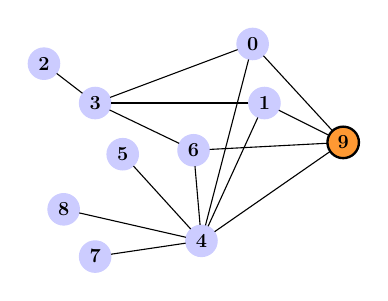
\begin{tikzpicture}[scale=0.5, transform shape,every node/.style={circle, draw, minimum size=8mm, font=\bfseries\Large}, 
                    every edge/.style={draw, thick=0.5mm}, 
                    node distance=1cm]
% Nodes
\node[fill=blue!20,draw=blue!20](0) at (0,0){0};
\node[fill=blue!20,draw=blue!20](1) at (0.3,-1.5){1};
\node[fill=blue!20,draw=blue!20](6) at (-1.5,-2.7){6};
\node[fill=blue!20,draw=blue!20](4) at (-1.3,-5){4};
\node[fill=orange!80,draw=black,line width=0.3mm](9) at (2.3,-2.5){9};
\node[fill=blue!20,draw=blue!20](3) at (-4,-1.5){3};
\node[fill=blue!20,draw=blue!20](5) at (-3.3,-2.8){5};
\node[fill=blue!20,draw=blue!20](8) at (-4.8,-4.2){8};
\node[fill=blue!20,draw=blue!20](2) at (-5.3,-0.5){2};
\node[fill=blue!20,draw=blue!20](7) at (-4,-5.4){7};

% % Edges
\draw (0) -- (9);
\draw (0) -- (4);
\draw (0) -- (3);
\draw (1) -- (3);
\draw (1) -- (9);
\draw (1) -- (4);
\draw (3) -- (6);
\draw (6) -- (9);
\draw (6) -- (4);
\draw (3) -- (2);
\draw (4) -- (8);
\draw (5) -- (4);
\draw (9) -- (4);
\draw (7) -- (4);

\end{tikzpicture}

    \caption{\small{Nine qubit graph state(blue) with one message qubit(orange).}}
    \label{fig:8 qubit cluster_9}
\end{figure}




\begin{table}[h]
\centering
\scriptsize
% \resizebox{0.4\textwidth}{!}{%
  % remove external padding so colored boxes touch vertical rules
  \setlength{\tabcolsep}{0pt} % IMPORTANT
  \renewcommand{\arraystretch}{1.4} % row height

  % Use simple centered columns; internal padding is handled by \PadCell / \PadCellColor
  \begin{tabular}{|c|c|c|c|}
    \hline
    \textbf{Data Error}  & \textbf{ Syndrome } & \textbf{ Data Error } & \textbf{ Syndrome } \\ \hline


    \rowcolor{gray!10}
    $Z_0$  & 10010100  & $Z_1$    &  10000000      \\ \hline
    $Z_2$  & 01000000  & $Z_3$    &  00100000      \\ \hline

    \rowcolor{gray!10}
    $Z_4$  & 00010000  & $Z_5$    &  00001000      \\ \hline
    $Z_6$  & 00000100  & $Z_7$    &  00000010      \\ \hline

    \rowcolor{gray!10}
    $Z_8$  & 00000001  & $X_0$    &  00110000      \\ \hline
    $X_1$  & 00110000  & $X_2$    &  00100000      \\ \hline

    \rowcolor{gray!10}
    $X_3$  & 01010000  & $X_4$    & 00011011       \\ \hline
    $X_5$  & 00010000  & $X_6$    &  00110000     \\ \hline

    \rowcolor{gray!10}
    $X_7$  & 00010000  & $X_8$    &  00010000      \\ \hline
    $Y_0$  & 10100100  & $Y_1$    &  10110000      \\ \hline

    \rowcolor{gray!10}
    $Y_2$  & 01100000  & $Y_3$    &  01110000      \\ \hline
    $Y_4$  & 00001011  & $Y_5$    &  00011000     \\ \hline

    \rowcolor{gray!10}
    $Y_6$  & 00110100  & $Y_7$    &   00010010     \\ \hline
    $Y_8$  & 00010001  &     &        \\ \hline


   

  \end{tabular}
% }
% }
\caption{Single-qubit error syndromes for the $[[9,1,3]]$ code}
\label{tab:errors_due_to_faults_9}
\end{table}

\begin{table}[h]
\centering
\scriptsize
% \resizebox{0.4\textwidth}{!}{%
  % remove external padding so colored boxes touch vertical rules
  \setlength{\tabcolsep}{0pt} % IMPORTANT
  \renewcommand{\arraystretch}{1.4} % row height

  % Use simple centered columns; internal padding is handled by \PadCell / \PadCellColor
  \begin{tabular}{|c|c|c|c|}
    \hline
    \textbf{ Data Error } & \textbf{ Syndrome } & \textbf{ Data Error } & \textbf{ Syndrome } \\ \hline

    % grey full-width multicolumn header (rowcolor applies to the multicolumn cell)
    \rowcolor{gray!20}
    \multicolumn{4}{|c|}{\boldmath\textbf{$Y_0 Z_1 Z_3 Y_4 Z_5 Z_6 Z_7Z_8$} $\longrightarrow$ $Z_1Y_4Y_0Z_5Z_3 Z_7Z_6Z_8$} \\ \hline

    % now rows; for yellow cells use \PadCellColor to ensure full coverage
    $Z_1X_4$  & 10011011  & $Z_1Y_4$    &  10001011      \\ \hline
    $Z_1YZ_4$  & 10010000  & $Z_1Y_4X_0$   &  10111011      \\ \hline
    $Z_1Y_4Y_0$  & 00101111  & $Z_1Y_4Z_0$    & 00011111      \\ \hline
    $Z_1Y_4Y_0X_5$  & 00111111  & $Z_1Y_4Y_0Y_5$    &  00110111      \\ \hline
    $Z_1Y_4Y_0Z_5$  & 00100111  & $Z_1Y_4Y_0Z_5X_3$    & 01110111      \\ \hline
    $Z_1Y_4Y_0Z_5Y_3$    &  01010111   & $Z_1Y_4Y_0Z_5Z_3$    &  00000111      \\ \hline
     $Z_1Y_4Y_0Z_5Z_3X_7$    &  00010111   & $Z_1Y_4Y_0Z_5Z_3Y_7$    &  00010101      \\ \hline

    $Z_1Y_4Y_0Z_5Z_3Z_7$    &  00000101   & $Z_1Y_4Y_0Z_5Z_3Z_7X_6$    &  00110101      \\ \hline

     $Z_1Y_4Y_0Z_5Z_3Z_7Y_6$    & 00110001   & &    \\ \hline


    
\rowcolor{gray!20}
    \multicolumn{4}{|c|}{\boldmath\textbf{$Z_0Z_1 Z_2 X_3Z_6$} $\longrightarrow$ $Z_0Z_2Z_1X_3Z_6$} \\ \hline

    % now rows; for yellow cells use \PadCellColor to ensure full coverage
   $Z_0X_2$  & 10110100  & $Z_0Y_2$    &  11110100      \\ \hline
   $Z_0Z_2$  & 11010100  & $Z_0Z_2X_1$    &  11100100      \\ \hline
   $Z_0Z_2Y_1$  & 01100100  & $Z_0Z_2Z_1$    &  01010100      \\ \hline
   $Z_0Z_2Z_1Y_3$  & 00100100  & $Z_0Z_2Z_1Z_3$    &  01110100      \\ \hline

  \end{tabular}
% }
\caption{Propagated errors in the $[[9,1,3]]$ code with their syndromes for the corresponding stabilizers.
The rearranging of stabilizers is illustrated in grey boxes. 
}
\label{tab:errors_due_to_faults_9_1}
\end{table}
\newpage
\subsection{[[10,1,3]] bare ancilla  code} 
Stabilizer generating set:
\begin{align}
& g_1= X_0 X_1,\   g_2 = X_2 Z_3, \  g_3=Z_0 Z_1 Z_2 X_3 Z_6, \ g_5=Z_4 X_5  \nonumber\\
 & g_4= Y_0 Z_1 Z_3 Y_4 Z_5 Z_6 Z_7Z_8Z_9,\   g_6=X_0 X_6, \ g_7=Z_4 X_7,\nonumber\\ &
\  g_8=Z_4X_8,\ g_9=Z_4X_9,
\label{eq:ten qubit generators}
\end{align}
Logical operators: 
\[ Z_l = X_0Z_2Z_4, \ \ \ X_l = Z_0Z_1Z_4Z_6.\]
\begin{figure}[h]
    \centering
    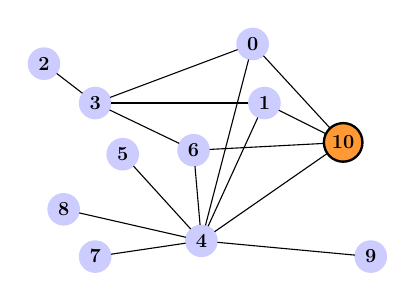
\begin{tikzpicture}[scale=0.5, transform shape,every node/.style={circle, draw, minimum size=8mm, font=\bfseries\Large}, 
                    every edge/.style={draw, thick=0.5mm}, 
                    node distance=1cm]
% Nodes
\node[fill=blue!20,draw=blue!20](0) at (0,0){0};
\node[fill=blue!20,draw=blue!20](1) at (0.3,-1.5){1};
\node[fill=blue!20,draw=blue!20](6) at (-1.5,-2.7){6};
\node[fill=blue!20,draw=blue!20](4) at (-1.3,-5){4};
\node[fill=orange!80,draw=black,line width=0.3mm](10) at (2.3,-2.5){10};
\node[fill=blue!20,draw=blue!20](3) at (-4,-1.5){3};
\node[fill=blue!20,draw=blue!20](5) at (-3.3,-2.8){5};
\node[fill=blue!20,draw=blue!20](8) at (-4.8,-4.2){8};
\node[fill=blue!20,draw=blue!20](2) at (-5.3,-0.5){2};
\node[fill=blue!20,draw=blue!20](7) at (-4,-5.4){7};
\node[fill=blue!20,draw=blue!20](9) at (3,-5.4){9};

% % Edges
\draw (0) -- (10);
\draw (0) -- (4);
\draw (0) -- (3);
\draw (1) -- (3);
\draw (1) -- (10);
\draw (1) -- (4);
\draw (3) -- (6);
\draw (6) -- (10);
\draw (6) -- (4);
\draw (3) -- (2);
\draw (4) -- (8);
\draw (5) -- (4);
\draw (10) -- (4);
\draw (7) -- (4);
\draw (4) -- (9);

\end{tikzpicture}

    \caption{\small{Ten qubit graph state(blue) with one message qubit(orange).}}
    \label{fig:8 qubit cluster_10}
\end{figure}




\begin{table}[h]
\centering
\scriptsize
% \resizebox{0.4\textwidth}{!}{%
  % remove external padding so colored boxes touch vertical rules
  \setlength{\tabcolsep}{0pt} % IMPORTANT
  \renewcommand{\arraystretch}{1.4} % row height

  % Use simple centered columns; internal padding is handled by \PadCell / \PadCellColor
  \begin{tabular}{|c|c|c|c|}
    \hline
    \textbf{Data Error}  & \textbf{ Syndrome } & \textbf{ Data Error } & \textbf{ Syndrome } \\ \hline


    \rowcolor{gray!10}
    $Z_0$  & 100101000  & $Z_1$    &  100000000      \\ \hline
    $Z_2$  & 010000000  & $Z_3$    &  001000000      \\ \hline

    \rowcolor{gray!10}
    $Z_4$  & 000100000  & $Z_5$    &  000010000      \\ \hline
    $Z_6$  & 000001000  & $Z_7$    &  000000100      \\ \hline

    \rowcolor{gray!10}
    $Z_8$  & 000000010  & $Z_9$ & 000000001 \\ \hline
    $X_0$  &  001100000   & $X_1$  & 001100000    \\ \hline

    \rowcolor{gray!10}
       $X_2$  &  001000000 &   $X_3$  & 010100000   \\ \hline
        $X_4$    & 000110111  &  $X_5$  & 000100000       \\ \hline
     

    \rowcolor{gray!10}
     $X_6$ &  001100000   &   $X_7$  & 000100000  \\ \hline
     $X_8$    &  000100000  & $X_9$ & 0001000000    \\ \hline
   
    \rowcolor{gray!10}
     $Y_0$  & 101001000  & $Y_1$    &  101100000      \\ \hline
    $Y_2$  & 011000000  & $Y_3$    &  011100000      \\ \hline
    

    \rowcolor{gray!10}
    $Y_4$  & 000010111  & $Y_5$    &  000110000     \\ \hline
    $Y_6$  & 001101000  & $Y_7$    &   000100100     \\ \hline
    
    \rowcolor{gray!10}
    $Y_8$  & 000100010  &     $Y_9$  & 000100011      \\ \hline


   

  \end{tabular}
% }
% }
\caption{Single-qubit error syndromes for the $[[10,1,3]]$ code}
\label{tab:errors_due_to_faults_10_1}
\end{table}

\begin{table}[ht]
\centering
\scriptsize

% \resizebox{0.4\textwidth}{!}{%
  % remove external padding so colored boxes touch vertical rules
  \setlength{\tabcolsep}{0pt} % IMPORTANT
  \renewcommand{\arraystretch}{1.4} % row height

  % Use simple centered columns; internal padding is handled by \PadCell / \PadCellColor
  \begin{tabular}{|c|c|c|c|}
    \hline
    \textbf{ Data Error } & \textbf{ Syndrome } & \textbf{ Data Error } & \textbf{ Syndrome } \\ \hline

    % grey full-width multicolumn header (rowcolor applies to the multicolumn cell)
    \rowcolor{gray!20}
    \multicolumn{4}{|c|}{\boldmath\textbf{$Y_0 Z_1 Z_3 Y_4 Z_5 Z_6 Z_7Z_8Z_9$} $\longrightarrow$ $Z_1Y_4Y_0Z_5Z_3 Z_7Z_6Z_8Z_9$} \\ \hline

    % now rows; for yellow cells use \PadCellColor to ensure full coverage
    $Z_1X_4$                    & 100110111    & $Z_1Y_4$                      &  100010111      \\ \hline
    $Z_1YZ_4$                   & 100100000    & $Z_1Y_4X_0$                   &  101110111      \\ \hline
    $Z_1Y_4Y_0$                 & 001011111    & $Z_1Y_4Z_0$                   &  000111111      \\ \hline
    $Z_1Y_4Y_0X_5$              & 001111111    & $Z_1Y_4Y_0Y_5$                &  001101111      \\ \hline
    $Z_1Y_4Y_0Z_5$              & 001001111    & $Z_1Y_4Y_0Z_5X_3$             &  011101111      \\ \hline
    $Z_1Y_4Y_0Z_5Y_3$           & 010101111    & $Z_1Y_4Y_0Z_5Z_3$             &  000001111      \\ \hline
    $Z_1Y_4Y_0Z_5Z_3X_7$        & 000101111    & $Z_1Y_4Y_0Z_5Z_3Y_7$          &  000101011      \\ \hline
    $Z_1Y_4Y_0Z_5Z_3Z_7$        & 000001011    & $Z_1Y_4Y_0Z_5Z_3Z_7X_6$       &  001101011      \\ \hline
    $Z_1Y_4Y_0Z_5Z_3Z_7Y_6$     & 001100011    & $Z_8Z_9$                      &  000000011   \\ \hline
    $X_8Z_9$                    & 000100001    & $Y_8Y_9$                      &  000100011  \\ \hline


    
\rowcolor{gray!20}
    \multicolumn{4}{|c|}{\boldmath\textbf{$Z_0Z_1 Z_2 X_3Z_6$} $\longrightarrow$ $Z_0Z_2Z_1X_3Z_6$} \\ \hline

    % now rows; for yellow cells use \PadCellColor to ensure full coverage
   $Z_0X_2$  & 10110100  & $Z_0Y_2$    &  11110100      \\ \hline
   $Z_0Z_2$  & 11010100  & $Z_0Z_2X_1$    &  11100100      \\ \hline
   $Z_0Z_2Y_1$  & 01100100  & $Z_0Z_2Z_1$    &  01010100      \\ \hline
   $Z_0Z_2Z_1Y_3$  & 00100100  & $Z_0Z_2Z_1Z_3$    &  01110100      \\ \hline

  \end{tabular}
\caption{Propagated errors in the $[[10,1,3]]$ code with their syndromes for the corresponding stabilizers.
The rearranging of stabilizers is illustrated in grey boxes. 
}
\label{tab:errors_due_to_faults_10_2}
\end{table}

\end{document}
%
% ****** End of file apssamp.tex ******
